
%%%%%%%% ICML 2026 EXAMPLE LATEX SUBMISSION FILE %%%%%%%%%%%%%%%%%

\documentclass{article}

% Recommended, but optional, packages for figures and better typesetting:
\usepackage{microtype}
\usepackage{graphicx}
\usepackage{subcaption}
\usepackage{booktabs} % for professional tables
\usepackage{multirow}
\usepackage{makecell}
% hyperref makes hyperlinks in the resulting PDF.
% If your build breaks (sometimes temporarily if a hyperlink spans a page)
% please comment out the following usepackage line and replace
% \usepackage{icml2026} with \usepackage[nohyperref]{icml2026} above.
\usepackage{hyperref}
\usepackage{siunitx}
\usepackage{float}

\usepackage{tikz}
  \usetikzlibrary{arrows.meta,positioning}
  
\sisetup{
  detect-weight=true,
  table-number-alignment=center,
  round-mode=places,
  round-precision=4
}

% Attempt to make hyperref and algorithmic work together better:
\newcommand{\theHalgorithm}{\arabic{algorithm}}

% Use the following line for the initial blind version submitted for review:
\usepackage{icml2026}

% For preprint, use
% \usepackage[preprint]{icml2026}

% If accepted, instead use the following line for the camera-ready submission:
% \usepackage[accepted]{icml2026}

\usepackage{amsmath}
\usepackage{amssymb}
\usepackage{mathtools}
\usepackage{amsthm}


% if you use cleveref..
\usepackage[capitalize,noabbrev]{cleveref}

%%%%%%%%%%%%%%%%%%%%%%%%%%%%%%%%
% THEOREMS
%%%%%%%%%%%%%%%%%%%%%%%%%%%%%%%%
\theoremstyle{plain}
\newtheorem{theorem}{Theorem}[section]
\newtheorem{proposition}[theorem]{Proposition}
\newtheorem{lemma}[theorem]{Lemma}
\newtheorem{corollary}[theorem]{Corollary}
\theoremstyle{definition}
\newtheorem{definition}[theorem]{Definition}
\newtheorem{assumption}[theorem]{Assumption}
\theoremstyle{remark}
\newtheorem{remark}[theorem]{Remark}

% Todonotes is useful during development; simply uncomment the next line
%    and comment out the line below the next line to turn off comments
\usepackage[disable,textsize=tiny]{todonotes}

% The \icmltitle you define below is probably too long as a header.
% Therefore, a short form for the running title is supplied here:
\icmltitlerunning{PP-Mark: Provable and Publicly Verifiable Watermarking for Generative AI}

\begin{document}

\twocolumn[
  \icmltitle{PP-Mark: Provable and Publicly Verifiable Watermarking for Generative AI}

  % It is OKAY to include author information, even for blind submissions: the
  % style file will automatically remove it for you unless you've provided
  % the [accepted] option to the icml2026 package.

  % List of affiliations: The first argument should be a (short) identifier you
  % will use later to specify author affiliations Academic affiliations
  % should list Department, University, City, Region, Country Industry
  % affiliations should list Company, City, Region, Country

  % You can specify symbols, otherwise they are numbered in order. Ideally, you
  % should not use this facility. Affiliations will be numbered in order of
  % appearance and this is the preferred way.
  \icmlsetsymbol{equal}{*}

  \begin{icmlauthorlist}
    \icmlauthor{}{}
    \icmlauthor{Firstname2 Lastname2}{equal,yyy,comp}
    \icmlauthor{Firstname3 Lastname3}{comp}
    \icmlauthor{Firstname4 Lastname4}{sch}
    \icmlauthor{Firstname5 Lastname5}{yyy}
    \icmlauthor{Firstname6 Lastname6}{sch,yyy,comp}
    \icmlauthor{Firstname7 Lastname7}{comp}
    %\icmlauthor{}{sch}
    \icmlauthor{Firstname8 Lastname8}{sch}
    \icmlauthor{Firstname8 Lastname8}{yyy,comp}
    %\icmlauthor{}{sch}
    %\icmlauthor{}{sch}
  \end{icmlauthorlist}

  \icmlaffiliation{yyy}{Department of XXX, University of YYY, Location, Country}
  \icmlaffiliation{comp}{Company Name, Location, Country}
  \icmlaffiliation{sch}{School of ZZZ, Institute of WWW, Location, Country}

  \icmlcorrespondingauthor{}{}
  \icmlcorrespondingauthor{}{}

  % You may provide any keywords that you find helpful for describing your
  % paper; these are used to populate the "keywords" metadata in the PDF but
  % will not be shown in the document
  \icmlkeywords{Machine Learning, ICML}

  \vskip 0.3in
]

% this must go after the closing bracket ] following \twocolumn[ ...

% This command actually creates the footnote in the first column listing the
% affiliations and the copyright notice. The command takes one argument, which
% is text to display at the start of the footnote. The \icmlEqualContribution
% command is standard text for equal contribution. Remove it (just {}) if you
% do not need this facility.

% Use ONE of the following lines. DO NOT remove the command.
% If you have no special notice, KEEP empty braces:
\printAffiliationsAndNotice{}  % no special notice (required even if empty)
% Or, if applicable, use the standard equal contribution text:
% \printAffiliationsAndNotice{\icmlEqualContribution}

\begin{abstract} 
Generative AI models now produce images indistinguishable from real data, making publicly verifiable provenance essential; however, existing watermarking methods become vulnerable to imprint forgeries and adversarial optimization attacks once their detectors are made public. We propose PP-Mark, a provenance framework that anchors lightweight statistical detection to a zero-knowledge proof of the embedding process, ensuring that forged content cannot pass full verification by construction. We establish formal unforgeability under standard cryptographic assumptions and validate PP-Mark against representative baselines across two architectures, demonstrating resistance to black-box imprint transfer, white-box optimization, and regeneration attacks while remaining practical for decentralized verification.
\end{abstract}


\section{Introduction}
The rapid proliferation of generative AI has made synthetic content increasingly indistinguishable from human-authored media, facilitating deepfakes, coordinated disinformation, and large-scale digital forgery \cite{chesney_citron2019}. This has created urgent demand for verifiable provenance that can be independently audited by the public \cite{longpre2024dataauth}. Industry-wide initiatives such as C2PA and regulatory frameworks including the EU AI Act now mandate explicit identification of AI-generated content \cite{c2pa_spec_2_3}, but the effectiveness of these standards depends on the robustness of the underlying technical mechanisms.

Digital watermarking is the leading approach for establishing provenance of generative content. Post-hoc methods embed signals in the pixel or frequency domain after generation (e.g., \cite{zhu2018hidden}), but remain vulnerable to regeneration and model-based attacks that can remove the embedded signal \cite{zhao2024removable}. Semantic watermarking mitigates this by injecting structured signals directly into the latent space during the generative process \cite{wen2023treerings,fernandez2023stablesignature,zhang2024zodiac}, exhibiting improved robustness against low-level manipulations.

Despite these advances, existing schemes exhibit a critical vulnerability. First, black-box imprint forgery attacks can extract watermark patterns from a single reference image and transfer them onto forged images by minimizing latent-space distances \cite{muller2025blackbox}. Second, when detectors $D(\cdot)$ are made public, they function as a differentiable or queryable loss, enabling adversaries to optimize forged content to satisfy the verification criterion directly \cite{jiang2023evading}. Public exposure of detection components can further enable surrogate-based optimization attacks that exceed conventional threat models \cite{lin2025crack}.

To mitigate these risks, existing systems rely on centralized verification, keeping $D(\cdot)$ private behind permissioned APIs. While this prevents leakage of the detection rule, it creates a trust bottleneck that precludes independent public auditing. The field thus faces a fundamental tension: private verification sacrifices public auditability, while public verification remains vulnerable to adversarial optimization. Recent work on privacy-preserving verification reflects this same tension \cite{guo2024zeromark}.

We resolve this tension by introducing PP-Mark (Provable Presence Mark), a provenance framework that is both publicly verifiable and resistant to forgery. Our key insight is to reformulate verification from a purely statistical inference problem into a cryptographically grounded proof. Rather than relying solely on a public detection score, which can be optimized against, PP-Mark anchors the verification rule to the specific generation context using zero-knowledge proofs (ZKP), ensuring that successful verification requires cryptographic consistency rather than detector manipulation.

We summarize our contributions as follows.
\begin{itemize}
    \item We introduce a context-bound latent embedding scheme and a zero-knowledge verification framework (based on SP1) that cryptographically anchors the detection rule to the generation context, enabling decentralized public verification without centralized APIs while preventing adversarial optimization for forgery.
    \item We prove formal unforgeability under standard cryptographic assumptions (Theorem~\ref{thm:unforgeability}) and evaluate against representative baselines across two model architectures.
\end{itemize}
  
\section{Related Works} 
\subsection{Watermarking Methods and Forgery Vulnerabilities}
Post-hoc methods such as HiDDeN \cite{zhu2018hidden}, StegaStamp \cite{tancik2020stegastamp}, TrustMark \cite{bui2023trustmark}, and InvisMark \cite{xu2024invismark} embed signals after generation for robust detection. Semantic approaches embed during generation: Tree-Ring \cite{wen2023treerings} and Gaussian Shading \cite{yang2024gaussianshading} modulate initial latent noise, while Stable Signature \cite{fernandez2023stablesignature}, DiffuseTrace \cite{lei2024diffusetrace}, and SFW \cite{lee2025iccv_sfw} strengthen resilience through decoder- or process-level injection. In the identification setting, RingID \cite{ci2024ringid} extends Tree-Ring to multi-key separability, WIND \cite{arabi2025wind} proposes a two-stage public detection pipeline, and MaXsive and TraceMark-LDM \cite{luo2025tracemarkldm,mao2025maxsive} push capacity. ISTS~\cite{zhong2024ists} strengthens forgery resistance through instance-specific injection and two-sided detection; PP-Mark pursues a complementary axis by cryptographically anchoring any detection rule to a verifiable proof rather than hardening the detector itself. However, these methods primarily target traceability and remain vulnerable to forgery and replay attacks that exploit exposed detection oracles \cite{jiang2023evading,muller2025blackbox}.

\subsection{Verifiable Computation}\label{sec:crypto-binding}
VeriLLM \cite{wang2025verillm} uses sampling-based commitments and randomized openings for publicly verifiable LLM inference checking; its ``good test'' property---that small random checks detect deviations with non-negligible probability---is analogous to PP-Mark's partial-opening bound (Theorem~\ref{thm:unforgeability}). PP-Mark adapts this commit-open-verify paradigm to image watermarking but additionally operates in zero knowledge and binds the opening set to the published image hash, preventing cross-image proof transfer.

\subsection{Undetectability and Content Provenance}
CLUE-Mark~\cite{shehata2024cluemark} embeds watermarks via the CLWE problem, providing provable \emph{undetectability}: an adversary without the secret key cannot distinguish watermarked from unwatermarked samples. PP-Mark targets a complementary property, provable \emph{unforgeability}, where any accepted image must have been produced by the legitimate generator; the two guarantees address orthogonal threat models and can in principle be combined. Unlike C2PA \cite{c2pa_spec_2_3}, which relies on certificate-based metadata signing, PP-Mark proves that a committed embedding trace is consistent with the public binding and anchored to the published image hash, a guarantee that signatures alone cannot provide.


  \begin{figure*}[t]
    \centering
    \includegraphics[width=\textwidth]{Approach2.pdf}
    \caption{PP-Mark overview. The generator embeds a latent watermark, commits sampled traces to a Merkle root, and produces a ZKP receipt. Verification uses latent inversion to compute a detection score and validates the receipt; acceptance requires both.}
    \label{fig:overview}
  \end{figure*}
  
\section{Method}
PP-Mark binds a latent-space watermark to the generation context and attaches a standalone SP1 zero-knowledge proof \cite{succinct2024sp1}. Provenance can be verified by any third party using only public artifacts, through a combination of a detection score and cryptographic proof verification.

\subsection{Overview and Threat Model}
We assume an adversary with access to watermarked images and public artifacts, who can perform arbitrary image manipulations. The adversary may attempt black-box imprint forgery or watermark removal attacks. However, the adversary does not possess the secret key and is assumed incapable of forging zero-knowledge proof receipts or breaking standard cryptographic hash functions.

\paragraph{Key Hierarchy.} PP-Mark distinguishes two independent keys to avoid confusion in forgery scenarios.
\begin{itemize}
  \item \textbf{Binding key $k$} (PP-Mark): a producer-held secret used to derive the binding value $b = \mathsf{H}(\texttt{ctx\_hash} \| h_{\mathrm{ctx}} \| k)$. The adversary does \emph{not} possess $k$; compromise of $k$ is outside our threat model and addressed separately via key rotation (see Sec.~\ref{sec:limitations}).
  \item \textbf{Metadata signing key $\mathrm{sk_{sig}}$} (baselines only): a standard digital-signature key used by the Sig-only and Sig+Score baselines (Sec.~\ref{sec:imprint-forgery}) to authenticate image metadata. $\mathrm{sk_{sig}}$ is \emph{independent} of $k$, and PP-Mark's unforgeability does \emph{not} depend on $\mathrm{sk_{sig}}$ secrecy. In forgery experiments the adversary may hold an arbitrary $\mathrm{sk_{sig}}$ (e.g., self-generated or stolen from a compromised platform) while still being blocked by the absence of $k$.
\end{itemize}

PP-Mark aims to (i) enable public, decentralized provenance verification without proprietary decoders or APIs, (ii) keep the binding key private while allowing third parties to verify correctness, (iii) prevent reuse or transfer by binding each watermark to the generation context, and (iv) maintain detectability under common transformations using a calibrated threshold \(\tau\) that controls false positives. Verification consists of two checks: watermark detection via a correlation score compared against \(\tau\), and validation of a ZKP receipt.

On the generation side, PP-Mark embeds a spread-spectrum watermark into the initial latent noise, commits sampled traces into a Merkle root \cite{merkle87}, and produces a ZKP receipt proving consistency between the binding and the commitment. The resulting metadata includes the context hash \(h_{\mathrm{ctx}}\), binding value \(b\), commitment root \(\mathrm{sample\_root}\), and audit parameters such as \(N\), \(\alpha_{\mathrm{eff}}\), the model identifier, and the LUT hash. The sample trace itself remains private and serves only as a proof witness.

On the verification side, a verifier performs latent inversion from the image, reconstructs the expected watermark signs from the public binding value \(b\), computes the detection score, and validates the ZKP receipt using public inputs. Because verification relies exclusively on public artifacts, PP-Mark enables decentralized provenance checks without proprietary decoders or centralized APIs, while the cryptographic proof prevents the verification rule from being exploited for forgery; the secret key never leaves the generator, yet any third party can independently verify provenance.

\subsection{Notation}
The generation context consists of a prompt $p$, random seed $s$, and model identifier $M$, with secret key $k$. The context hash is denoted by $h_{\mathrm{ctx}}$, and the corresponding public binding value by $b$. The truncated message is $m$, encoded as a Reed–Solomon codeword $c$ and expanded into a bitstream $\mathtt{bits}$. The latent grid is $Z \in \mathbb{R}^{H \times W \times 4}$, indexed by $i$ or equivalently $(x,y,\mathrm{ch})$. The inverse-CDF lookup table is $F^{-1}$. A deterministic sample set $S$ of size $|S|=N$ is used for watermark embedding. For each sampled index, $g_i$ denotes the Gaussian baseline and $z_i$ the corresponding watermarked latent. We denote the normalized initial latent as $z^{(0)}$, and the latent recovered via DDIM inversion as $\hat{z}^{(0)}$. The effective watermark strength is $\alpha_{\mathrm{eff}}$.

For provenance verification, $s_i \in {-1,+1}$ denotes the expected sign pattern and $r_i$ the recovered residual. The sampled trace is denoted by $\mathcal{T}$ and committed to the Merkle root $\mathrm{sample\_root}$. The final detection score is $\mathrm{score}$ with threshold $\tau$, and the SP1 zero-knowledge proof receipt is denoted by $\pi$. We define the image hash $h_{\mathrm{img}} = \mathsf{SHA\text{-}256}(\mathtt{pixels}(I))$, computed over the raw pixel bytes of the generated image $I$. The opening challenge seed is defined as
$\mathrm{challenge\_seed} = \mathrm{SHA256}(x)$ where $x = \mathrm{domain} \,\|\, h_{\mathrm{img}} \,\|\, h_{\mathrm{ctx}} \,\|\, \mathrm{sample\_root}$. Openings correspond to a deterministic subset of the existing trace, denoted by $K \subseteq S$ with $|K| = k \ll N$. The commitment to the openings is given by the digest $\mathrm{opening\_digest}$. The opening check verifies that each opened trace entry satisfies the deterministic embedding relation derived from $b$ ($\mathcal{P}_4$; see Theorem~\ref{thm:unforgeability}).



%%%%%%  
%\begin{table}[t]
%\centering
%\caption{Core symbols used throughout the method}
%\label{tab:notation}
%\begin{tabular}{ll}
%\hline
%Symbol & Meaning \\
%  \hline
%  $p, s, M$ & prompt, seed, model id \\
%  $k, h_{\mathrm{ctx}}, b$ & secret key, context hash, binding value \\
%  $m, c, \mathtt{bits}$ & message, RS codeword, bitstream \\
%  $Z$ & latent grid $Z \in \mathbb{R}^{H \times W \times 4}$ \\
%  $z^{(0)}, \hat{z}^{(0)}$ & normalized and inverted latents \\
%  $F^{-1}$ & inverse-CDF LUT \\
%  $S, N$ & sample set and count ($N=1000$) \\
%  $K, k_{\mathrm{open}}$ & opening subset and count ($k_{\mathrm{open}} \ll N$) \\
%  $h_{\mathrm{img}}$ & normalized image hash \\
%  $\mathrm{challenge\_seed}$ & hash-derived opening seed \\
%  $\mathrm{opening\_digest}$ & commitment to openings \\
%  $\alpha, \alpha_{\mathrm{eff}}$ & watermark strength (raw, effective) \\
%%  $s_i, r_i$ & expected signs and recovered residuals \\
%%  $\mathrm{sample\_root}$ & Merkle root of sampled trace $\mathcal{T}$ \\
%%  $\mathrm{score}, \tau, \pi$ & score, threshold, SP1 receipt \\
%%\hline
%%\end{tabular}
%%\end{table}


\subsection{Binding and Payload}\label{sec:binding-payload}
PP-Mark binds each watermark to the full generation context so that reuse or transfer under a different setting is detectable. We first hash the prompt and then construct a context hash using domain separation:
\begin{equation}
h_p = \mathsf{H}(p)
\end{equation}

\begin{equation}
h_{\mathrm{ctx}} = \mathsf{H}(\texttt{ctx\_hash} \,\|\, h_p \,\|\, M \,\|\, s \,\|\, W \,\|\, H)
\end{equation}

The public binding value is derived from the context hash and the secret key:
\begin{equation}
b = \mathsf{H}(\texttt{ctx\_hash} \,\|\, h_{\mathrm{ctx}} \,\|\, k)
\label{eq:binding_relation}
\end{equation}

Let \(u = (h_{\mathrm{img}}, h_{\mathrm{ctx}}, \mathrm{sample\_root})\). The opening challenge seed is defined as
\begin{equation}
\mathrm{challenge\_seed} = \mathsf{H}(\texttt{ppmark\_opening\_v1} \,\|\, u).
\end{equation}

The proof additionally commits to an opening digest derived from \(\mathrm{challenge\_seed}\), corresponding to a deterministic subset of the sampled trace.

Any change in the prompt, model, seed, or resolution yields a different binding value \(b\), preventing cross-context reuse. From \(b\), we derive a fixed-length payload \(m = \mathrm{Trunc}(b)\) and apply Reed--Solomon encoding to obtain a codeword \(c\). The codeword is expanded into a binary sequence \(\mathtt{bits}\) that drives deterministic sampling and embedding. Reed--Solomon encoding provides a stable seed for sampling, while decoding is used only for diagnostic purposes.

\subsection{Deterministic Sampling and Bit Mapping}
To bound the proof cost, PP-Mark verifies only a fixed subset of latent positions. The sample
set is deterministically derived from the public codeword:
\begin{equation}
S = \mathrm{DeterministicSample}(c, N).
\end{equation}

For each spatial coordinate \((x,y)\), a bit index is deterministically selected from the
binding value:
\begin{equation}
\mathrm{idx}(x,y) = \mathsf{H}(b \,\|\, x \,\|\, y \,\|\, 777) \bmod L,
 L = |\mathtt{bits}|.
\end{equation}

We further select a deterministic opening subset \(K \subseteq S\) of size
\(k_{\mathrm{open}} = 32\) using \(\mathrm{challenge\_seed}\). This mapping spreads the payload across the latent grid and supports robust detection under mild distortions. Because \(S\) is derived from the public codeword \(c\), any verifier can reproduce the same sampled positions, keeping the proof cost bounded while preserving public verifiability.
  

\subsection{Watermark Embedding}\label{sec:embedding}
For each latent index \(i\), a pseudo-random uniform value \(u_i\) is generated from the
binding value \(b\) and mapped to a Gaussian baseline \(g_i\) via an inverse-CDF lookup
table:
\begin{equation}
u_i = \mathsf{H}(b \,\|\, i{+}1) \bmod 2^{32},
\quad
g_i = F^{-1}\!\left( \frac{u_i}{2^{32}} \right).
\end{equation}

Each spatial position is indexed as \(i=(x,y)\) on a fixed reference channel. A payload bit
is mapped to a sign \(s_i \in \{-1,+1\}\), and the watermark is injected into the baseline:
\begin{equation}
s_i = 2 \cdot \mathtt{bits}_{\mathrm{idx}(x,y)} - 1,
\quad
z_i = g_i + \alpha s_i.
\end{equation}

To maintain stable latent variance and ensure that the embedding remains within the
expected distribution of the pre-trained model, we apply the following normalization:
\begin{equation}
z_i^{(0)} = \frac{z_i}{\sqrt{1+\alpha^2}},
\quad
\alpha_{\mathrm{eff}} = \frac{\alpha}{\sqrt{1+\alpha^2}}.
\end{equation}

This normalization stabilizes the detection score distribution and reduces sensitivity to
global rescaling, a common scale-based perturbation. For sampled indices \(i \in S\), we
record the tuple \((i, g_i, z_i^{(0)}, \mathrm{bit})\) as a sample trace and commit it using a Merkle
tree (Fig.~\ref{fig:merkle}). Here both $g_i$ and the post-normalization value $z_i^{(0)}$ are stored in a fixed-point encoding (Q18) so that all circuit-side arithmetic is exact, and the effective amplitude is $\alpha_{\mathrm{eff}} = \alpha/\sqrt{1+\alpha^2}$. The resulting \(\mathrm{sample\_root}\) is published as part of
the public metadata and serves as a cryptographic anchor. This hierarchical commitment
ensures that any adversarial manipulation of the private latent witness results in
verification failure during ZKP receipt validation, as the trace remains a private
foundational witness for the SP1 proof.


\begin{figure}[t]
  \centering
  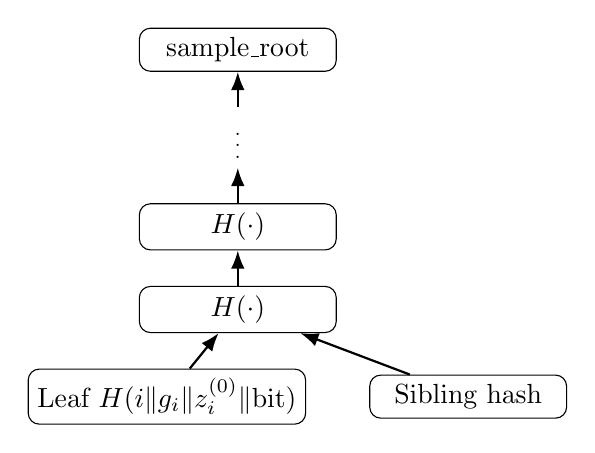
\begin{tikzpicture}[
    box/.style={draw, rounded corners, align=center, minimum width=2.5cm, minimum height=0.5cm},
    node distance=0.45cm and 0.8cm
  ]
  \node[box] (leafL) {Leaf $H(i \| g_i \| z_i^{(0)} \| \mathrm{bit})$};
  \node[box, right=of leafL] (leafR) {Sibling hash};
  \node[box, above=of leafL, xshift=0.9cm] (h1) {$H(\cdot)$};
  \node[box, above=of h1] (h2) {$H(\cdot)$};
  \node[above=of h2] (dots) {\scriptsize$\vdots$};
  \node[box, above=of dots] (root) {$\mathrm{sample\_root}$};

  \draw[-Latex, thick] (leafL) -- (h1);
  \draw[-Latex, thick] (leafR) -- (h1);
  \draw[-Latex, thick] (h1) -- (h2);
  \draw[-Latex, thick] (h2) -- (dots);
  \draw[-Latex, thick] (dots) -- (root);
  \end{tikzpicture}
  \caption{Merkle authentication path for a sampled trace element used as a proof witness.}
  \label{fig:merkle}
\end{figure}

\subsection{SP1 Proof Generation}
PP-Mark leverages the SP1 zkVM \cite{succinct2024sp1} to generate a standalone zero-knowledge proof receipt \(\pi\). The proof establishes, in zero knowledge, that the published binding value \(b\) and the committed sampled trace \(\mathcal{T}\), anchored by \(\mathrm{sample\_root}\), are consistent with a valid secret key \(k\) and payload \(\mathtt{bits}\), without revealing these secrets.

We adopt SP1 for engineering practicality: its Rust-based tooling and parallelizable proving architecture enable efficient integration into high-throughput generative pipelines. The circuit \(\mathcal{C}\) does not re-simulate the full diffusion process, but it does enforce all relations necessary to cryptographically bind the committed trace to the public binding value $b$: it verifies that $b$ is derived from a valid secret key (P1), that the full trace is Merkle-committed (P2), that the opening digest is consistent with an image-derived challenge (P3), and that on randomly opened positions, the baseline $g_i$ and payload bit $\mathtt{bit}_i$ are deterministically derived from $b$ and the embedding relation $z_i^{(0)} = g_i + \alpha_{\mathrm{eff}} \cdot s_i$ holds exactly (P4). Since $b$ deterministically governs the entire sign pattern through the chain $b \to c \to \mathtt{bits} \to s_i$ (Sec.~\ref{sec:binding-payload}--\ref{sec:embedding}), verifying this chain on the opened subset anchors the full detection pipeline without incurring the cost of re-executing the embedding across all $N$ positions.

\subsubsection{Statement and Witness}
The SP1 proof \(\pi\) attests to the existence of a private witness \(w\) that satisfies the
verification predicate with respect to a public statement \(x\).

\begin{definition}
  \textbf{(Public Statement \(x\))}
  The public statement consists of the binding value \(b\), the commitment root
  \(\mathrm{sample\_root}\), the opening digest \(\mathrm{opening\_digest}\), the opening size
  \(k_{\mathrm{open}}\), and auxiliary verification metadata such as the Merkle tree depth.
  The LUT hash $\mathsf{H}(F^{-1})$ is included in $x$ and enforced by the circuit when verifying $g_i$ on opened positions ($\mathcal{P}_4$). The sampling size $N$ is public for auditability.
\end{definition}

\begin{definition}
  \textbf{(Private Witness \(w\))}
The private witness contains sensitive generation data, including the secret key \(k\),
the Reed--Solomon codeword \(c\), and the sampled trace
\(\mathcal{T} = \{(i, g_i, z_i^{(0)}, \mathrm{bit})\}_{i \in S}\) (with $g_i, z_i^{(0)}$ in fixed-point) together with the corresponding Merkle authentication paths.
\end{definition}

\textbf{Circuit Constraints.}
The circuit \(\mathcal{C}\) enforces four groups of constraints (formalized as $\mathcal{P}_1$--$\mathcal{P}_4$ in Sec.~\ref{thm:unforgeability}):
(i)~the binding value is correctly computed as \(b = \mathsf{H}(\texttt{"ctx\_hash"} \,\|\, h_{\mathrm{ctx}} \,\|\, k)\);
(ii)~each leaf in the sampled trace \(\mathcal{T}\) reconstructs the committed \(\mathrm{sample\_root}\) via its Merkle authentication path;
(iii)~the opening positions are derived from \(\mathrm{challenge\_seed}\) and the recomputed \(\mathrm{opening\_digest}\) matches the public digest; and
(iv)~for each opened index $i \in K$, the circuit re-derives the Reed--Solomon codeword $c$ from $b$, extracts $\mathtt{bit}_i$ at the corresponding index, computes $g_i = F^{-1}[\mathsf{H}(b \,\|\, i{+}1) \bmod 2^{32}]$ using the committed LUT hash, and verifies $z_i^{(0)} = g_i + \alpha_{\mathrm{eff}} \cdot (2\mathtt{bit}_i - 1)$ in Q18 fixed-point arithmetic.
Constraint~(iv) ensures that the committed trace entries on the opened subset are not arbitrary but follow the deterministic embedding procedure governed by~$b$.

The resulting receipt \(\pi\) is standalone and publicly verifiable. Since forging \(\pi\) is computationally infeasible without access to the secret key \(k\) and a trace consistent with the $b$-derived embedding, the proof ensures that knowledge of the public detector alone is insufficient to fabricate valid provenance.

\subsection{Extraction and Verification}
Given an image, its associated metadata, and an SP1 receipt, the verifier performs DDIM
inversion to recover an approximate latent representation \(\hat{z}^{(0)}\). The verifier
computes the image hash \(h_{\mathrm{img}} = \mathsf{SHA\text{-}256}(\texttt{pixels}(I))\), derives
\(\mathrm{challenge\_seed}\), and validates the opening subset \(K\) against the metadata
digest; this opening check is incorporated into
\(\text{VerifyReceipt}(\pi; x)\), where the image enters only through its hash (Algorithm~\ref{alg:verify}). The verifier then reconstructs \(m\), \(c\), and
\(\mathbf{bits}\) from the public binding value \(b\), regenerates the sample set \(S\), and
derives the expected sign pattern.

\begin{assumption}[Statistical Properties of Inversion Residuals]
\label{assum:noise}
Let \(\epsilon_i = \hat{z}_i - z_i\) denote the DDIM inversion residual at latent index \(i\).
We assume that \(\epsilon_i\) follows an approximately zero-mean distribution, i.e.,
\(\mathbb{E}[\epsilon_i] \approx 0\), and has bounded moderate correlation with the
watermark signal \(s_i\).
\end{assumption}

The residual correlation arises from signal attenuation during the VAE encode--decode cycle: the lossy pixel-space roundtrip partially absorbs the watermark perturbation, inducing a negative correlation between \(\epsilon\) and \(s\). Empirically, the mean \(|\rho(\epsilon, s)|\) is \(0.30\) on SD\,2.1 and \(0.54\) on SDXL across 100 images each (Appendix~\ref{app:assumption-verify}); the larger magnitude on SDXL reflects its \(4{\times}\) larger latent grid, which increases inversion error at a fixed DDIM step count. In both cases the correlation is bounded well below~1 and its sign is consistently negative, so the attenuation is a multiplicative shrinkage rather than a source of score collapse. Empirically the clean detection score remains at least \(5{\times}\) above the threshold \(\tau\) on every image in both models (SD\,2.1: mean score~\(25.7\), \(\mathrm{score}/\tau \approx 10\); SDXL: mean score~\(13.6\), \(\mathrm{score}/\tau \approx 5.5\)), confirming that this attenuation does not compromise detection reliability.

Under Assumption~\ref{assum:noise}, for each sampled index \(i \in S\) the recovered
latent value is \(\hat{z}_i = z_i + \epsilon_i\), where \(z_i = g_i + \alpha_{\mathrm{eff}}\, s_i\). Defining the expected watermark signal \(w_i = \alpha_{\mathrm{eff}}\, s_i\), the inner product
\(\langle \hat{z}_S, w_S \rangle = \alpha_{\mathrm{eff}}^2 \|s_S\|^2 + \langle g_S, w_S\rangle + \langle \epsilon_S, w_S\rangle\).
Because \(g\) and \(s\) are derived from independent hash chains, \(\langle g_S, w_S\rangle \approx 0\) in expectation.
\label{eq:residual}

PP-Mark uses \(N = 1000\) samples to compute the final detection score. This choice balances
statistical stability, reducing score variance through averaging, against the proving and
verification overhead of the SP1 pipeline. The detection score is defined as the normalized
correlation over the sample set \(S\):
\begin{equation}
\mathrm{score}
= \frac{|\langle \hat{z}_S,\, w_S \rangle|}{\|w_S\|}.
\end{equation}

The score measures the alignment between the recovered residuals \(r_S\) and the expected
sign pattern \(s_S\). Finally, an image is accepted as authentic if and only if it satisfies
both the statistical and cryptographic verification criteria:

\begin{equation}
{\small
\text{Accept}(I,\pi)\iff (\mathrm{score}\ge\tau)\land(\text{VerifyReceipt}(\pi; x)=1).
}
\end{equation}


\begin{algorithm}[t]
\caption{Verify and Extract}
\label{alg:verify}
\begin{algorithmic}[1]
\STATE Input:
\parbox[t]{0.85\linewidth}{
image \(I\), metadata \(\mathrm{md}\) (including \(h_{\mathrm{ctx}}, b,
\mathrm{sample\_root}, \mathrm{opening\_digest}, k_{\mathrm{open}}\)), receipt \(\pi\)
}
\STATE \(\hat{z}^{(0)} \leftarrow \text{DDIM\_Inversion}(I)\)
\STATE Reconstruct \(\mathbf{bits}\) from \(b\); regenerate sample set \(S\) from \(c\)
\FOR{each \(i \in S\)}
  \STATE \(g_i \leftarrow F^{-1}(\mathsf{H}(b \,\|\, i{+}1) \bmod 2^{32})\)
  \STATE \(w_i \leftarrow \alpha_{\mathrm{eff}} \cdot s_i\) where \(s_i = 2 \cdot \mathbf{bits}_{\mathrm{idx}(i)} - 1\)
\ENDFOR
\STATE \(\mathrm{score} \leftarrow \frac{|\langle \hat{z}_S,\, w_S \rangle|}{\|w_S\|}\)
\STATE \(h_{\mathrm{img}} \leftarrow \mathsf{SHA\text{-}256}(\texttt{pixels}(I))\) \COMMENT{image enters proof only via hash}
\STATE \(\texttt{proof\_ok} \leftarrow \text{VerifyReceipt}(\pi; \mathrm{md}, h_{\mathrm{img}})\)
\STATE Return \((\mathrm{score} \ge \tau) \land \texttt{proof\_ok}\)
\end{algorithmic}
\end{algorithm}

  
\subsection{Synchronization and Security Rationale}
To handle transformation-induced misalignment, PP-Mark employs an alignment search over
latent positions. A central efficiency--security trade-off arises from our use of
deterministic sampling with \(N=1000\), since verifying the full latent space within a ZKP
circuit would be computationally prohibitive for real-time deployment. Under bounded and
approximately independent samples, empirical averages concentrate in the Hoeffding sense
\cite{hoeffding1963}, enabling high-throughput verification while preserving the
statistical reliability required for stable detection.

Furthermore, the binding value \(b\) ties the watermark to the full generation context,
ensuring that any modification to the prompt or random seed induces a distinct
commitment. By anchoring statistical detection to a ZKP receipt \(\pi\), the detection
score becomes contingent on a valid cryptographic proof rather than on the score alone.
As a result, even if an adversary optimizes a forgery to achieve a high detection score,
verification fails in the absence of a consistent latent trace and proof, which cannot be
constructed without access to the secret witness.

Crucially, the statistical and cryptographic layers are not independent but share a common trust anchor. The score check derives its discriminative power from the sign pattern $s_i$, which is deterministically keyed by $b$. Without assurance that $b$ was legitimately derived, an adaptive adversary could fabricate a binding $b'$ whose induced sign pattern maximizes the score for an arbitrary target image. The ZKP provides exactly this assurance: it certifies that $b$ originates from a valid secret key and generation context, foreclosing the fabricated-binding attack (formalized in Theorem~\ref{thm:unforgeability}). Conversely, the score layer contributes what the proof alone cannot: it statistically links the \emph{image latent} to the $b$-derived sign pattern, providing graceful degradation under lossy transforms (Appendix~\ref{Image Transformations}). The circuit deliberately does not compare opened trace values to image-derived latents; instead, the image enters the proof solely through $h_{\mathrm{img}}$ in the challenge seed ($\mathcal{P}_3$), which binds the opening set $K$ to the specific published image and prevents cross-image proof transfer. The statistical comparison between image and trace is handled by the score, whose discriminative power is anchored to $b$ by the circuit. The two layers thus address complementary threat surfaces through the same cryptographic foundation.

This complementarity motivates two operational modes. \textbf{PP-Mark(score)} performs statistical detection only: it verifies $\mathrm{score} \geq \tau$ in milliseconds and suffices for large-scale, routine provenance screening where the generator is trusted. \textbf{PP-Mark(accept)} additionally verifies the ZKP receipt $\pi$, incurring a one-time proving cost (${\sim}48$\,s) but providing cryptographic non-repudiation for legal evidence, regulatory compliance (e.g., the EU AI Act), and scenarios where the generator itself may be untrusted. Table~\ref{tab:threat-coverage} summarizes the threat coverage of each mode; Section~\ref{sec:sig-vs-zkp} validates this distinction experimentally. In return, score mode offers two practical advantages that accept mode lacks: robustness to lossy transforms such as JPEG compression and rescaling (Appendix~\ref{Image Transformations}), and sub-second verification latency suitable for high-throughput content platforms (Table~\ref{tab:runtime}).

\begin{table}[t]
\centering
\caption{Threat coverage by verification mode. In score mode the verifier trusts that the generator embedded honestly: a malicious generator could fabricate a binding $b'$ whose induced sign pattern exceeds $\tau$ on an unwatermarked image (Table~\ref{tab:sig-vs-zkp}). Accept mode blocks this via ZKP verification of the $b{\to}\mathtt{bits}{\to}z$ derivation chain.}
\label{tab:threat-coverage}
\small
\begin{tabular}{lcc}
\toprule
Threat model & Score & Accept \\
\midrule
External adversary (unknown $k$) & \checkmark & \checkmark \\
Generator fraud (no embedding) & $\times$ & \checkmark \\
Third-party audit (no $k$ disclosure) & $\times$ & \checkmark \\
\bottomrule
\end{tabular}
\end{table}

\paragraph{Image canonicalization for $h_{\mathrm{img}}$.}
Before hashing, the image is canonicalized deterministically: EXIF orientation is normalized (\texttt{exif\_transpose}), the pixel buffer is forced to 8-bit RGB, resampled to the model-native resolution with bicubic interpolation, and quantized to $\{0,\dots,255\}$ via round-and-clip. SHA-256 is then applied to the resulting byte array, so $h_{\mathrm{img}}$ is invariant only to trivial metadata/format differences while remaining sensitive to every pixel-level change.

We use a cryptographic hash for $h_{\mathrm{img}}$ rather than a perceptual hash to prevent \emph{proof replay}: a perceptual hash maps visually similar but distinct images to the same digest, which would allow an attacker to reuse a legitimate proof $\pi$ for a manipulated image $I'$ sharing the same perceptual hash. SHA-256 ensures that any pixel-level modification invalidates the challenge seed and thus the opening verification. This design choice yields a strict trade-off: legitimate benign edits (recompression, mild crop, resizing) also break the receipt, so the generator must re-issue a proof over the re-published image. Re-proving is tractable (\,$\sim\!48\,$s at $N{=}1000$, Table~\ref{tab:runtime}\,) and is performed once per edited variant, mirroring how C2PA manifests are reissued on edits. A robust perceptual hash (e.g., LSH over a pretrained encoder) could relax this requirement, but it would open an explicit proof-replay window equal to the hash's collision neighborhood, which we deliberately avoid.

\subsection{Formal Security Guarantee}

\begin{assumption}\label{asm:crypto}
SHA-256 is collision-resistant, and the SP1 zkVM satisfies computational soundness with respect to security parameter $\lambda$.
\end{assumption}

\paragraph{Composite verification predicate.}
Let $x=(b, \mathrm{sample\_root}, \mathrm{opening\_digest}, \mathrm{challenge\_seed}, k_{\mathrm{open}}, \alpha_{\mathrm{eff}}, h_{\mathrm{ctx}})$ denote the public statement, and let $w=(k, c, \mathcal{T}, \mathrm{paths})$ denote the private witness with $\mathcal{T}=\{(i,g_i,z_i^{(0)},\mathtt{bit}_i)\}_{i \in S}$. The SP1 circuit $\mathcal{C}$ enforces the composite predicate $\mathcal{P}(x, w) = \bigwedge_{j=1}^{4} \mathcal{P}_j(x, w)$:
\begin{align*}
\mathcal{P}_1&: b = \mathsf{H}(\texttt{ctx\_hash} \,\|\, h_{\mathrm{ctx}} \,\|\, k), \\
\mathcal{P}_2&: \forall i \in S,\; \mathrm{FoldMerkle}(\mathrm{leaf}_i, \mathrm{paths}_i) = \mathrm{sample\_root}, \\
\mathcal{P}_3&: \mathrm{opening\_digest} = \mathsf{H}\!\left( \{\mathrm{leaf\_tuple}_i\}_{i \in K} \right), \\
&\text{where } K = \mathrm{DeriveOpen}(\mathrm{challenge\_seed}, k_{\mathrm{open}}, N), \\
\mathcal{P}_4&: \forall i \in K,\;
  \mathtt{bit}_i = \mathrm{RS}(b)[\mathrm{idx}(i)], \;\;
  g_i = F^{-1}\!\bigl[\mathsf{H}(b \,\|\, i{+}1) \bmod 2^{32}\bigr], \\
  &\qquad\qquad\; z_i^{(0)} = g_i + \alpha_{\mathrm{eff}} \cdot (2\mathtt{bit}_i - 1) \pmod{\text{Q18}}.
\end{align*}
Clause $\mathcal{P}_1$ binds the committed $b$ to possession of $k$; $\mathcal{P}_2$ commits the full trace; $\mathcal{P}_3$ forces the adversary to commit \emph{before} seeing which positions will be checked (since $\mathrm{challenge\_seed} = \mathsf{H}(\texttt{ppmark\_opening\_v1} \| h_{\mathrm{img}} \| h_{\mathrm{ctx}} \| \mathrm{sample\_root})$); and $\mathcal{P}_4$ enforces that on the $k_{\mathrm{open}}$ opened positions, the payload bit and Gaussian baseline are deterministically derived from $b$ (via Reed--Solomon decoding and the committed inverse-CDF LUT), and that the stored latent satisfies the exact embedding relation. This prevents an adversary from committing arbitrary trace entries that satisfy the arithmetic relation tautologically.

\begin{theorem}[Unforgeability under composite predicate and partial opening]\label{thm:unforgeability}
Under Assumption~\ref{asm:crypto}, for any probabilistic polynomial-time adversary $\mathcal{A}$ that does not possess the secret key $k$ and commits a trace with at least $q$ positions violating the honest embedding relation,
\begin{align*}
\Pr[&\mathrm{PP\text{-}Mark}_{\mathrm{accept}}(I^*, \mathrm{md}^*, \pi^*) = 1 \;\wedge\; (I^*, \pi^*) \notin \mathcal{G}] \\
&\leq \; \mathrm{Adv}^{\mathrm{cr}}_{\mathsf{H}}(\mathcal{A}) + \mathrm{Adv}^{\mathrm{sound}}_{\mathrm{SP1}}(\mathcal{A}) + \binom{N-q}{k_{\mathrm{open}}} \big/ \binom{N}{k_{\mathrm{open}}},
\end{align*}
where $\mathcal{G}$ is the set of image-proof pairs legitimately produced by the generator and the last term is bounded by $(1 - q/N)^{k_{\mathrm{open}}}$.
\end{theorem}

\begin{proof}[Proof sketch; full reduction in Appendix~\ref{app:full-proof}]
Acceptance requires both (i)~$\mathrm{score} \geq \tau$ and (ii)~$\mathrm{VerifyReceipt}(\pi^*; \mathrm{md}^*, h_{\mathrm{img}}^*) = 1$; it suffices to bound~(ii). By SP1 computational soundness, a verifying $\pi^*$ implies a witness $w^*$ satisfying $\mathcal{P}_1$--$\mathcal{P}_4$, except with probability $\mathrm{Adv}^{\mathrm{sound}}_{\mathrm{SP1}}(\mathcal{A})$.

\emph{Binding forgery.} $\mathcal{P}_1$ requires $b = \mathsf{H}(\texttt{ctx\_hash}\,\|\,h_{\mathrm{ctx}}\,\|\,k^*)$ for some $k^*$ encoded in the witness. Producing $k^* \neq k$ that yields the target $b$ requires a SHA-256 preimage/collision, contributing $\mathrm{Adv}^{\mathrm{cr}}_{\mathsf{H}}(\mathcal{A})$.

\emph{Trace forgery (full).} $\mathcal{P}_2$ commits the entire trace $\mathcal{T}$ via Merkle authentication; after publishing $\mathrm{sample\_root}$ the adversary cannot change any tuple without an SHA-256 collision.

\emph{Partial opening.} By $\mathcal{P}_3$, the opening set $K$ is derived deterministically from $\mathrm{challenge\_seed} = \mathsf{H}(\texttt{ppmark\_opening\_v1}\,\|\,h_{\mathrm{img}}\,\|\,h_{\mathrm{ctx}}\,\|\,\mathrm{sample\_root})$; because $\mathrm{sample\_root}$ is fixed before $h_{\mathrm{img}}$ is known (and vice-versa, since $h_{\mathrm{img}}$ is the hash of the published image), the adversary cannot adaptively align $K$ with the cheating positions. Viewing $K$ as a uniform $k_{\mathrm{open}}$-subset of $\{1,\ldots,N\}$, the probability that $K$ avoids the $q$ cheating positions is $\binom{N-q}{k_{\mathrm{open}}}/\binom{N}{k_{\mathrm{open}}} \leq (1-q/N)^{k_{\mathrm{open}}}$. Conditioned on $K$ hitting at least one cheating position (where $\mathtt{bit}_i$, $g_i$, or the embedding equation deviates from the $b$-derived values), $\mathcal{P}_4$ detects the violation with probability $1$.

\emph{Image-binding.} $h_{\mathrm{img}}$ enters $\mathrm{challenge\_seed}$ via $\mathcal{P}_3$, so transferring a valid proof from $I_A$ to $I^* \neq I_A$ changes $K$ and invalidates the opening digest, unless $\mathsf{H}$ is inverted.

Summing the three failure modes yields the stated bound.
\end{proof}

\paragraph{Parameter choice and remaining guarantees.} With $N=1000$ and $k_{\mathrm{open}}=32$, the partial-opening term evaluates to $(1 - q/N)^{32} \approx 2^{-6.3}$ at $q = 0.125 N$ (12.5\% cheating), meaning the adversary evades the opening check with probability ${\approx}1.3\%$; equivalently, 32 random spot-checks detect the violation with probability ${\geq}98.7\%$. The bound tightens rapidly: at $q = 0.25 N$ it drops to ${\approx}2^{-13}$, and at $q = 0.5 N$ to $2^{-32}$. An adversary cheating on fewer positions gains at most proportionally small influence on the detection score; the remaining soundness gap is absorbed by the score threshold $\tau$ (calibrated at $1\%$~FPR), yielding a two-layer defence: large-$q$ cheating is caught cryptographically by the opening, and small-$q$ cheating is caught statistically by $\tau$. The opening-tolerance parameter $\varepsilon$ in $\mathcal{P}_4$ is set to $0$ at Q18 fixed-point precision (i.e., exact equality), made tight by synthesizing $\mathrm{combined\_fixed}_i = g_i + \alpha_{\mathrm{eff}} \cdot (2\mathtt{bit}_i - 1)$ from $(g_i, \mathtt{bit}_i)$ in the opening digest itself; enlarging $\varepsilon$ would additively widen the forger's advantage by the fraction of $2\varepsilon$-neighbouring latent values and is therefore avoided in our instantiation.

\section{Experiments}
\subsection{Experimental Setup}
We use Stable Diffusion v2.1 base with a DDIM scheduler, 50 inference steps, and guidance scale 7.5. PP-Mark uses $\alpha=4.0$, sample count $N=1000$, and SHA-256 sampling for SP1. Prompts are drawn from the Stable-Diffusion-Prompts dataset. All methods are calibrated to the same 1\% FPR on clean(non-watermarked) images using their native detection statistics. We calibrate on clean SD2.1 images generated under the same settings.
Table~\ref{tab:runtime} reports end-to-end runtime for each method.

\begin{table}[t]
\centering
\caption{Runtime comparison (H100 PCIe, SD2.1, 512$\times$512).
Semantic methods embed during diffusion generation; post-hoc methods apply a separate encoder to the generated image.}
\label{tab:runtime}
\small
\begin{tabular}{lcc}
\toprule
Method & Embed (s) & Verify (s) \\
\midrule
Tree-Ring & 0.89 & 0.75 \\
Gaussian Shading & 3.10 & 0.72 \\
RingID & 0.89 & 0.72 \\
WIND & 0.89 & 1.10 \\
Stable Signature & 0.91 & 0.008 \\
HiDDeN & 0.001 & 0.001 \\
TrustMark & 0.013 & 0.004 \\
InvisMark & 0.002 & 0.009 \\
\midrule
PP-Mark (score) & 0.89 & 0.72 \\
PP-Mark (accept) & 0.89\,{+}\,48.6$^{\dagger}$ & 0.72\,{+}\,7.59$^{\dagger}$ \\
\bottomrule
\end{tabular}
\vspace{2pt}

{\footnotesize $^{\dagger}$ZKP prove\,/\,verify overhead ($N{=}1000$, SP1 zkVM).}
\vskip -0.1in
\end{table}

\paragraph{Receipt artifacts.} \label{sec:proof-size}
For $N{=}1000$, the PP-Mark receipt consists of a compact public-input header (666\,B: binding, sample root, opening digest, challenge seed, $k_{\mathrm{open}}$, Merkle depth, and $\alpha_{\mathrm{eff}}$) and the SP1 STARK proof ($\approx\!40.7$\,MB). The private witness used only for proving is $\approx\!922$\,KB. Size scales near-linearly with $N$: $12.2/16.9/24.8/40.7/66.0$\,MB for $N\in\{300,400,600,1000,1500\}$; a full sweep is tabulated in Appendix~\ref{app:proof-size}. A STARK-to-SNARK wrapper stage (future work) would further reduce receipt bandwidth to the tens-of-kilobytes range at a one-time proving cost, matching C2PA manifest budgets.

\subsection{Verification Ablation}\label{sec:sig-vs-zkp}

To validate the necessity of zero-knowledge verification (Table~\ref{tab:threat-coverage}), we compare four verification architectures under two targeted attacks on $n=100$ watermarked images at FPR\,=\,1\%:

\begin{itemize}
\item \textbf{Forged binding.} An adversary who controls only the metadata signing key $\mathrm{sk_{sig}}$ (but \emph{not} the PP-Mark binding key $k$) fabricates a binding $b'$ to maximize the detection score for a target image. We evaluate $10{,}000$ random bindings per image (sufficient to expect ${\sim}70$ scores exceeding $\tau$ under the null per-trial probability of ${\approx}0.7\%$) and report the fraction for which the best score exceeds $\tau$.
\item \textbf{Compliance bypass.} An adversary generates a clean (unwatermarked) image and signs legitimate-looking metadata without embedding any watermark signal.
\end{itemize}

\begin{table}[t]
\centering
\caption{Forgery Acceptance Rate (FAR) under two attacks across four verification architectures ($n=100$, FPR\,=\,1\%).}
\label{tab:sig-vs-zkp}
\small
\begin{tabular}{lcccc}
\toprule
Attack & Sig-only & Sig+Score & \makecell{PP-Mark\\(score)} & \makecell{PP-Mark\\(accept)} \\
\midrule
Forged binding & 1.00 & 1.00 & ${\leq}$0.01$^{\dagger}$ & \textbf{0.00} \\
Compliance bypass & 1.00 & 0.00 & ${\leq}$0.01$^{\dagger}$ & \textbf{0.00} \\
\bottomrule
\end{tabular}
\vspace{2pt}

{\footnotesize $^{\dagger}$Upper-bounded by FPR; 0/100 observed. Binding $b$ is cryptographically fixed by the secret key.}
\end{table}

Table~\ref{tab:sig-vs-zkp} reports the results. A signature-only system is trivially defeated by both attacks (FAR\,=\,1.00). Adding a score threshold blocks compliance bypass but not forged binding: random search over $10{,}000$ candidate bindings consistently finds at least one whose induced sign pattern exceeds $\tau$ (mean best score $3.88 \gg \tau{=}2.47$). PP-Mark(score) resists both attacks because the binding is cryptographically fixed by the generator's secret key $k$, leaving the adversary no degree of freedom. PP-Mark(accept) provides the strongest guarantee: the ZKP rejects any fabricated binding regardless of the achieved score, confirming Theorem~\ref{thm:unforgeability} empirically.

\subsection{Imprint Forgery Attack}\label{sec:imprint-forgery}
Imprint forgery is a strong black-box and method-agnostic threat: from a
single watermarked reference image, an attacker attempts to transfer the watermark imprint onto an arbitrary cover so the verifier attributes it to the same source
\cite{muller2025blackbox}. This captures a realistic adversary who does not know the target watermark design but can adapt a proxy generator, making it a practical strong attack. We use SD2.1 for both the target and the proxy in the imprint-forgery attack. To evaluate this threat fairly, we construct a fixed prompt pool (200 prompts; 100/100 calibration/evaluation) and prepare a cover pool of 100 images as targets for attribution transfer. We fix 100 cover–reference pairs (one reference per cover) and reuse the same pairs across all methods to avoid pairing bias.

\subsubsection{Direct Imprint Forgery}
We apply the standard imprint-forgery optimizer to each fixed cover--reference pair and evaluate with each method’s native detector (Forgery Acceptance Rate(FAR)@1\%(False Positive Rate(FPR), $n=100$ per step).
Table~\ref{tab:direct-vulnerability} reports results for Tree-Ring and Gaussian Shading \cite{yang2024gaussianshading} as a sanity check of the attack pipeline; both are highly vulnerable(TR: 0.92→0.97, GS: 1.00 across steps).


\sisetup{
  detect-weight=true,
  table-number-alignment=center,
  round-mode=places,
  round-precision=2
}

  \begin{table}[t]
    \caption{Direct vulnerability under targeted imprint forgery.
    FAR@1\%FPR (targeted verify); All methods evaluated at FPR=1\% (clean-calibrated)}
    \label{tab:direct-vulnerability}
    \begin{center}
      \begin{small}
        \begin{sc}
          \begin{tabular}{
          c
          S[table-format=1.3, round-mode=none] S[table-format=1.3, round-mode=none]
          }
            \toprule
            &
            \multicolumn{1}{c}{\textbf{TR}} &
            \multicolumn{1}{c}{\textbf{GS}} \\
            \cmidrule(lr){2-2}\cmidrule(lr){3-3}
            \textbf{Step}
            & {\textbf{FAR@1\%FPR}} & {\textbf{FAR@1\%FPR}} \\
            \midrule
            50 & 0.92 & 1.00 \\
            100 & 0.97 & 1.00 \\
            150 & 0.97 & 1.00 \\
            Avg. & 0.953 & 1.00 \\
            \bottomrule
          \end{tabular}
        \end{sc}
      \end{small}
    \end{center}
    \vskip -0.1in
  \end{table}

  \begin{table}[t]
      \caption{Transfer results by method and step.
      FAR@1\%FPR (targeted verify); All methods evaluated at FPR=1\% (clean-calibrated). TrustMark and InvisMark use bit-accuracy as the continuous score (see text).}
      \label{tab:transfer-steps}
      \begin{center}
        \begin{small}
          \begin{sc}
            \resizebox{\linewidth}{!}{%
            \begin{tabular}{
            l c
            S[table-format=1.2] S[table-format=1.2]
            }
              \toprule
              & &
              \multicolumn{1}{c}{\textbf{TR}} &
              \multicolumn{1}{c}{\textbf{GS}} \\
              \cmidrule(lr){3-3}\cmidrule(lr){4-4}
              \textbf{Method} & \textbf{Step}
              & {\textbf{FAR@1\%FPR}} & {\textbf{FAR@1\%FPR}} \\
              \midrule

              \multirow{3}{*}{TrustMark} & 50 & 0.05 & 0.01 \\
                                        & 100 & 0.03 & 0.02 \\
                                        & 150 & 0.03 & 0.05 \\
                \addlinespace

              \multirow{3}{*}{InvisMark} & 50 & 0.06 & 0.03 \\
                                         & 100 & 0.01 & 0.01 \\
                                         & 150 & 0.02 & 0.01 \\
                \addlinespace

              \multirow{3}{*}{RingID} & 50 & 0.01 & 0.01 \\
                                        & 100 & 0.10 & 0.02 \\
                                        & 150 & 0.01 & 0.01 \\
                \addlinespace

                \multirow{3}{*}{StableSig} & 50 & 0.04 & 0.01 \\
                                           & 100 & 0.04 & 0.02 \\
                                           & 150 & 0.02 & 0.02 \\
                \addlinespace

                \multirow{3}{*}{HiDDeN} & 50 & 0.04 & 0.01 \\
                                        & 100 & 0.02 & 0.03 \\
                                        & 150 & 0.01 & 0.03 \\
                \addlinespace

                \multirow{3}{*}{WIND} & 50 & 0.01 & 0.01 \\
                                     & 100 & 0.01 & 0.01 \\
                                     & 150 & 0.01 & 0.01 \\
                \addlinespace

                \multirow{3}{*}{PP-Mark$_{\mathrm{score}}$} & 50 & 0.00 & 0.00 \\
                                         & 100 & 0.00 & 0.01 \\
                                         & 150 & 0.01 & 0.01 \\
                \addlinespace

                \multirow{3}{*}{PP-Mark$_{\mathrm{accept}}$} & 50 & 0.00 & 0.00 \\
                                         & 100 & 0.00 & 0.00 \\
                                         & 150 & 0.00 & 0.00 \\

              \bottomrule
            \end{tabular}}
          \end{sc}
        \end{small}
      \end{center}
      \vskip -0.1in
    \end{table}



\begin{table*}[t]
    \caption{Transfer summary over steps.
    FAR@1\%FPR (targeted verify) with 95\% CI.
    All methods evaluated at FPR=1\% (clean-calibrated).
    $\Delta$\% is computed as $(k-k_{\mathrm{PP\text{-}Mark_{score}}})/k_{\mathrm{PP\text{-}Mark_{score}}} \times 100$, where $k_{\mathrm{PP\text{-}Mark_{score}}}=1$ (TR) and $k_{\mathrm{PP\text{-}Mark_{score}}}=2$ (GS). Fisher $p$ is from a one-sided Fisher exact test vs PP-Mark$_{\mathrm{score}}$ (H1: method $>$ PP-Mark$_{\mathrm{score}}$).}
    \label{tab:transfer-summary}
    \begin{center}
      {\scriptsize
      \setlength{\tabcolsep}{2pt}
      \renewcommand{\arraystretch}{1}
        \begin{sc}
          
          \begin{tabular}{
          l
          S[table-format=1.4, round-mode=places, round-precision=4, round-pad=true] c c c
          S[table-format=1.4, round-mode=places, round-precision=4, round-pad=true] c c c
          }
            \toprule
            & \multicolumn{4}{c}{\textbf{TR}} & \multicolumn{4}{c}{\textbf{GS}} \\
            \cmidrule(lr){2-5}\cmidrule(lr){6-9}
            \textbf{Method} & {\textbf{FAR@1\%FPR}} & \textbf{95\% CI} & \textbf{$\Delta$\%} &
  \textbf{Fisher $p$}
            & {\textbf{FAR@1\%FPR}} & \textbf{95\% CI} & \textbf{$\Delta$\%} & \textbf{Fisher $p$} \\
            \midrule
            TrustMark & 0.0367 & 0.0184--0.0647 & +1000.0 & 0.0029 & 0.0267 & 0.0116--0.0519 & +300.0 & 0.0532 \\
            InvisMark & 0.0300 & 0.0133--0.0500 & +800.0 & 0.0102 & 0.0167 & 0.0033--0.0333 & +150.0 & 0.2252 \\
            RingID & 0.0400 & 0.0208--0.0688 & +1100.0 & 0.0016 & 0.0133 & 0.0036--0.0338 & +100.0 &
  0.3430 \\
            StableSig & 0.0333 & 0.0161--0.0604 & +900.0 & 0.0055 & 0.0167 & 0.0054--0.0385 & +150.0 &
  0.2252 \\
            HiDDeN & 0.0233 & 0.0094--0.0475 & +600.0 & 0.0343 & 0.0233 & 0.0094--0.0475 & +250.0 & 0.0882
  \\        WIND & 0.0100 & 0.0021--0.0289 & +200.0 & 0.3119 & 0.0100 & 0.0021--0.0289 & +50.0 & 0.5000 \\
            PP-Mark$_{\mathrm{score}}$ & 0.0033 & 0.0001--0.0184 & -- & -- & 0.0067 & 0.0008--0.0239 & -- & -- \\
            PP-Mark$_{\mathrm{accept}}$ & 0.0000 & -- & -- & -- & 0.0000 & -- & -- & -- \\            
            \bottomrule
          \end{tabular}
        \end{sc}
      }
    \end{center}
    \vskip -0.1in
  \end{table*}
  
  \subsubsection{Transfer Imprint Forgery} 
  We evaluate cross-method vulnerability to the standard imprint-forgery pipeline. Tree-Ring (TR) and Gaussian Shading (GS) are used as canonical imprint sources to keep the attack fixed across methods. For each fixed cover--reference pair, we extract the imprint from a single TR/GS-watermarked reference and optimize it onto the cover. All detectors are evaluated under thresholds calibrated to 1\% FPR on clean images, so differences reflect detector susceptibility under the same fixed pairings and step budget.(PP‑Mark$_{\mathrm{score}}$ reports score-only acceptance for cross-method comparability, while PP‑Mark$_{\mathrm{accept}}$ enforces the full verification rule.)
  
  Since TrustMark's \cite{bui2023trustmark} and InvisMark's \cite{xu2024invismark} public APIs return only binary detection flags with no tunable threshold, we use \emph{bit accuracy}---the fraction of correctly decoded payload bits---as a continuous score, enabling standard FPR=1\% calibration on clean images (TrustMark: $\tau{=}0.58$, clean ${\approx}0.48$, watermarked ${\approx}1.00$; InvisMark: $\tau{=}0.49$, clean ${\approx}0.41$, watermarked ${\approx}0.96$).

  Table~\ref{tab:transfer-steps} reports step-wise transfer success for each method when the imprint source is TR or GS. PP‑Mark$_{\mathrm{score}}$ remains at 0.00--0.01 across steps, indicating that the standard imprint-forgery pipeline rarely pushes it beyond its calibrated false-positive floor. TrustMark, InvisMark, and other baselines (RingID, StableSignature, HiDDeN) exceed this floor, showing materially higher susceptibility under identical calibration and attack conditions.
  
  \subsubsection{Summary of Transfer Imprint Forgery}
Table~\ref{tab:transfer-summary} summarizes transfer acceptance rates aggregated across the three optimization steps under a fixed pairing protocol. Across both TR- and GS-sourced imprints, PP‑Mark$_{\mathrm{score}}$ consistently attains the lowest acceptance rates, effectively remaining at or below the 1\% calibration floor (0.0033 for TR and 0.0067 for GS). This indicates that the imprint-forgery attack fails to move PP-Mark’s score beyond the statistical noise floor of a clean image. In contrast, RingID, Stable Signature, and HiDDeN exhibit substantially higher transfer acceptance under TR-sourced attacks, with point estimates an order of magnitude larger than PP‑Mark$_{\mathrm{score}}$. 

The $\Delta\%$ column reports ratios computed from raw counts relative to PP‑Mark$_{\mathrm{score}}$’s small denominators. While these ratios appear numerically large, they are intended as descriptive summaries rather than primary effect size. The absolute FARs and their $95\%$ confidence intervals therefore provide the appropriate basis for comparison and consistently rank PP‑Mark$_{\mathrm{score}}$ as the least susceptible method under the same calibration and attack conditions. 

One-sided Fisher exact tests against PP‑Mark$_{\mathrm{score}}$ further support this ordering for TR-sourced imprints: the higher acceptance rates of RingID, Stable Signature, and HiDDeN are statistically significant ($p=0.0016$, $0.0055$, and $0.0343$, respectively). For GS-sourced imprints, the differences do not reach statistical significance at the $0.05$ level. Nevertheless, the point estimates and confidence intervals preserve the same practical ordering, with PP‑Mark$_{\mathrm{score}}$ remaining the least vulnerable among all evaluated methods.

\begin{figure}[t]
    \centering
    \includegraphics[width=1\linewidth]{transfer forest(WIND).pdf}
    \caption{Cross-method transfer at FPR=1\%. Error bars denote 95\% CI; the vertical line indicates PP-Mark$_{\mathrm{score}}$.}
    \label{fig:transfer-forest}
\end{figure}

\subsection{White-Box Forgery Attack}
We consider a strongest case white-box adversary with full access to each detector and
gradients, optimizing inputs to maximize the detection score under an $\ell_\infty$ budget $\epsilon=2/255$ using $T=150$ PGD steps. For each method, forgery acceptance is defined by $\mathrm{score}\ge\tau$, where $\tau$ is calibrated at 1\% FPR. In contrast, PP‑Mark$_{\mathrm{accept}}$ requires passing both statistical and cryptographic checks. 

All methods are attacked via their differentiable pipelines: TrustMark, InvisMark, Stable Signature, and HiDDeN use differentiable decoders; RingID and PP‑Mark$_{\mathrm{score}}$ use differentiable inversion-based scores. For WIND, we optimize a differentiable Fourier-distance surrogate while evaluating against the actual detector.

Table~\ref{tab:white-box-summary} shows outcomes across methods. All baselines reach FAR@1\%FPR = 1.00, with RingID, TrustMark, and InvisMark being the fastest to break (2.26, 2.41, and 3.07 steps, respectively), while PP-Mark$_{\mathrm{score}}$ remains lower (0.76).  PP‑Mark$_{\mathrm{score}}$ attains a lower FAR but a smaller mean step among accepted cases
than WIND. This is consistent with the objective structure: PP‑Mark uses a keyed, image‑conditioned correlation/bit‑sign score (sample indices and sign map vary per image), which can yield highly variable progress, some images align quickly while others stall. WIND uses a fixed pattern/mask reconstruction objective shared across images, which promotes more uniform progress and thus more consistent acceptance, typically at later steps on average. Thus, PP‑Mark’s faster successes reflect higher variance rather than overall weakness, whereas WIND trades slightly slower convergence for near‑certain acceptance. Figure~\ref{fig:wb_forge_far_curves} shows the cumulative FAR trajectories across steps. 
  
\begin{table}[t]
  \caption{White-Box forgery outcomes across methods. FAR@1\%FPR is the forgery acceptance rate. Avg.\ Steps to FA reports, among forgery acceptances, the mean optimization step (within a fixed budget of 150 steps) at which $\mathrm{score}\ge\tau$ first occurs. PSNR is averaged against the original cover image.}
  \label{tab:white-box-summary}
  \begin{center}
    {\footnotesize
    \setlength{\tabcolsep}{2pt}
    \renewcommand{\arraystretch}{1}
      \begin{sc}
        \begingroup
        \hypersetup{hidelinks}
        \begin{tabular}{
          l
          S[table-format=1.2, round-mode=places, round-precision=2, round-pad=true]
          S[table-format=3.2, round-mode=places, round-precision=2, round-pad=true]
          S[table-format=2.2, round-mode=places, round-precision=2, round-pad=true]
        }
          \toprule
          \textbf{Method}
          & {\makecell{\textbf{FAR}\\ \textbf{@1\%FPR}}}
          & {\makecell{\textbf{Avg.\ }\\ \textbf{Steps to FA}}}
          & {\makecell{\textbf{Avg.\ }\\ \textbf{PSNR $\uparrow$}}} \\
          \midrule
          TrustMark                 & 1.00 & 2.41  & 75.73 \\
          InvisMark                 & 1.00 & 3.07  & 72.67 \\
          StableSig                 & 1.00 & 5.40  & 65.91 \\
          HiDDeN                    & 1.00 & 8.08  & 62.96 \\
          RingID                    & 1.00 & 2.26  & 74.51 \\
          WIND                      & 1.00 & 22.20 & 55.76 \\
          PP-Mark$_{\mathrm{score}}$  & 0.76 & 17.42 & 67.69 \\
          PP-Mark$_{\mathrm{accept}}$ & 0.00 & \multicolumn{1}{c}{--} & \multicolumn{1}{c}{--} \\          \bottomrule
        \end{tabular}
        \endgroup
      \end{sc}
    }
  \end{center}
  \vskip -0.1in
\end{table}

\begin{figure}[H]
    \centering
    \includegraphics[width=1\linewidth]{wb_forge_far_curves.pdf}
    \caption{Cumulative FAR@1\%FPR vs. optimization step for all methods under the same attack budget and evaluation setup.}
    \label{fig:wb_forge_far_curves}
\end{figure}

For PP-Mark$_{\mathrm{accept}}$, watermark acceptance requires proof verification. The
attacked image changes the image hash $h_{\mathrm{img}}$, which changes 
$\mathrm{challenge\_seed}$ and thus the opening positions and the recomputed 
$\mathrm{opening\_digest}$. As a result, the verifier’s opening check and proof verification fails, PP‑Mark$_{\mathrm{accept}}$ stays at FAR=0.

\subsection{Removal Attacks}
We assess PP-Mark’s resilience to watermark erasure at a fixed detection threshold (FPR=1\%), focusing on whether signals can be removed without compromising image quality.

\subsubsection{Regeneration Attack}
The adversary employs diffusion-based re-synthesis to wash out the watermark while preserving visual content \cite{zhao2024removable}. PP-Mark remains highly detectable at all noise steps (TPR 0.98), whereas StableSig and HiDDeN drop to 0.01–0.06. InvisMark is the most vulnerable, collapsing to near-random bit accuracy (TPR${\le}0.05$) even at the weakest noise step, while TrustMark shows intermediate robustness (0.85 at 30 steps) but degrades to 0.39 at 100 steps. Both pixel-space methods are progressively washed out by re-synthesis, in contrast to PP-Mark's latent-space embedding which survives intact. We evaluate survival rates across varying noise intensities; detailed configurations and per-step results are provided in Appendix~\ref{sec:Regeneration Attack}.

\subsubsection{Steganalysis Attack}
This attack estimates and subtracts the watermark signal using $K$ reference samples. PP-Mark stays highly detectable as K increases (TPR 0.864–0.963), whereas Tree-Ring drops to 0.02–0.038 and StableSig stays around 0.17–0.20. Full results for various $K$ are detailed in Appendix~\ref{Steganalysis Attack}.

\subsection{Image Transformations}
We evaluate watermark robustness under standard pixel-level and geometric transformations.
PP-Mark retains high detection for JPEG, blur, noise, and brightness changes (0.86--1.00),
remains robust to random crop + resize (SD\,2.1: 0.87; SDXL: 0.74),
and recovers from large rotations via a fine-grained rotation-sync search
(rotation $75^\circ$: SD\,2.1 0.85; SDXL 0.97).
Full results are in Appendix~\ref{Image Transformations} (Table~\ref{tab:image-transforms}).

\subsection{Generation Distributional Fidelity}
We assess distributional fidelity using KID (an unbiased metric) between clean and watermarked image sets; full results are provided in Appendix~\ref{Generation Distributional Fidelity}.

\section{Limitations}\label{sec:limitations}
\paragraph{ZKP overhead.} PP-Mark's decentralized verification relies on a SP1 STARK receipt whose size and proving time scale with the sample count $N$ (${\approx}40.7$\,MB and ${\approx}48.6$\,s at $N{=}1000$; Table~\ref{tab:runtime}, App.~\ref{app:proof-size}). This is tolerable for archival or on-request verification but costly for per-upload streaming pipelines; a STARK-to-SNARK wrapper or proof aggregation are natural reductions that we leave to future work.

\paragraph{Key lifecycle.} PP-Mark's unforgeability is contingent on the producer's binding key $k$ remaining secret; if $k$ leaks, the adversary can mint valid receipts under the victim's identity. We treat this as an operational security requirement and recommend the following lifecycle, consistent with standard PKI practice: (i)~\emph{rotation}---each producer maintains a small set of active binding keys $\{k^{(t)}\}$ indexed by a rotation epoch $t$; metadata includes the current key identifier, so verifiers can tell which epoch a receipt belongs to; (ii)~\emph{revocation}---a compromised $k^{(t)}$ is published on a public revocation list (analogous to CRL/OCSP), and verifiers reject receipts bound to revoked epochs; (iii)~\emph{forward binding}---because $b$ only depends on the \emph{context} at generation time, rotated keys do not invalidate legitimate historical receipts as long as the corresponding epoch remains non-revoked. Integration with C2PA Content Credentials is straightforward: the epoch ID, rotation policy, and revocation URL can be carried as standard assertion fields.

\paragraph{Geometric robustness.} Rotation is largely recovered through a dedicated rotation-sync search (step $0.25^\circ$, LANCZOS4 interpolation), retaining $0.85/0.97$ (SD\,2.1/SDXL) at $75^\circ$; random crop on SDXL (0.74) is the remaining soft spot due to higher sub-pixel sensitivity of the $128{\times}128$ latent (App.~\ref{Additional Limitations and Discussions}). We confirm security properties generalize to SDXL (App.~\ref{app:sdxl}). Additional limitations and discussions are continued in Appendix~\ref{Additional Limitations and Discussions}.

\section{Conclusion}
PP-Mark leverages public zero-knowledge proof to enable decentralized verification of AI-generated provenance, while substantially reducing susceptibility to forgery attack. By anchoring the context-bound detection score to a publicly verifiable cryptographic proof, PP-Mark demonstrates that decentralized, open verification can coexist with robust resistance to state-of-the-art forgery attack. We hope this work lays a foundation for transparent and robust provenance verification of AI-generated content.

\section*{Impact Statement}
This work provides a decentralized, verifiable mechanism for AI image provenance, helping reduce misattribution and synthetic media misuse. By removing reliance on centralized APIs and addressing forgery threats, PP-Mark enables transparent auditing of provenance claims under clear operational assumptions. We view this as a technical building block that complements broader socio-technical efforts for the responsible deployment of generative AI.



\bibliography{example_paper}
\bibliographystyle{icml2026}

%%%%%%%%%%%%%%%%%%%%%%%%%%%%%%%%%%%%%%%%%%%%%%%%%%%%%%%%%%%%%%%%%%%%%%%%%%%%%%%
%%%%%%%%%%%%%%%%%%%%%%%%%%%%%%%%%%%%%%%%%%%%%%%%%%%%%%%%%%%%%%%%%%%%%%%%%%%%%%%
% APPENDIX
%%%%%%%%%%%%%%%%%%%%%%%%%%%%%%%%%%%%%%%%%%%%%%%%%%%%%%%%%%%%%%%%%%%%%%%%%%%%%%%
%%%%%%%%%%%%%%%%%%%%%%%%%%%%%%%%%%%%%%%%%%%%%%%%%%%%%%%%%%%%%%%%%%%%%%%%%%%%%%%

\clearpage

\appendix
\section{Full Proof of Theorem~\ref{thm:unforgeability}}\label{app:full-proof}

We give the step-by-step reduction for Theorem~\ref{thm:unforgeability} (conditions on $\mathcal{A}$ and $q$ are as stated in the main text).

\paragraph{Security game.} Let $\mathcal{G}$ be the set of $(I, \pi)$ pairs produced by honest \textsf{Generate}. $\mathcal{A}$ is given the SP1 verification key, the public statement $x$ of one honestly-generated image, and oracle access to $\mathsf{H}=\mathrm{SHA\text{-}256}$; it wins by outputting $(I^*, \mathrm{md}^*, \pi^*)$ such that PP-Mark accepts and $(I^*, \pi^*) \notin \mathcal{G}$. We bound $\Pr[\mathcal{A}\text{ wins}]$ via four failure modes plus a union bound.

\paragraph{Witness extraction.} By computational soundness of SP1 with parameter $\lambda$~\cite{succinct2024sp1}, whenever $\pi^*$ verifies on public statement $x^*$, there exists (except with probability $\mathrm{Adv}^{\mathrm{sound}}_{\mathrm{SP1}}(\mathcal{A})$) a witness $w^* = (k^*, c^*, \mathcal{T}^*, \mathrm{paths}^*)$ such that the composite predicate $\mathcal{P}_1 \wedge \mathcal{P}_2 \wedge \mathcal{P}_3 \wedge \mathcal{P}_4$ holds on $(x^*, w^*)$. We condition on successful extraction henceforth.

\paragraph{Case A: Binding forgery ($k^* \neq k$ with reused $b$).} Suppose $\mathcal{A}$ reuses the honest $b$ in $x^*$ but the extracted witness carries $k^* \neq k$. By $\mathcal{P}_1$, $b = \mathsf{H}(\texttt{ctx\_hash} \,\|\, h_{\mathrm{ctx}}^* \,\|\, k^*)$, while the honest $b$ equals $\mathsf{H}(\texttt{ctx\_hash} \,\|\, h_{\mathrm{ctx}} \,\|\, k)$; $\mathcal{A}$ has thus exhibited an SHA-256 second-preimage for $b$. Case~A contributes at most $\mathrm{Adv}^{\mathrm{cr}}_{\mathsf{H}}(\mathcal{A})$.

\paragraph{Case B: Merkle trace forgery.} $\mathcal{P}_2$ requires each leaf $\mathrm{leaf}_i = \mathsf{H}(i, g_i, z_i^{(0)}, \mathtt{bit}_i)$ to reconstruct $\mathrm{sample\_root}^*$ via the standard Merkle authentication path~\cite{merkle87}. If $\mathcal{A}$ reuses $\mathrm{sample\_root}$ from the honest run but alters any tuple in $\mathcal{T}^*$, reconstructing the same root requires a SHA-256 collision on some ancestor node; union-bounding over the $\log_2 N$ tree edges is absorbed into $\mathrm{Adv}^{\mathrm{cr}}_{\mathsf{H}}(\mathcal{A})$.

\paragraph{Case C: Partial opening with $q$ cheating positions.} Let $F \subseteq S$ be the set of indices at which $\mathcal{T}^*$ violates the full embedding relation enforced by $\mathcal{P}_4$: index $i \in F$ iff $\mathtt{bit}_i \neq \mathrm{RS}(b^*)[\mathrm{idx}(i)]$, or $g_i \neq F^{-1}[\mathsf{H}(b^* \,\|\, i{+}1) \bmod 2^{32}]$, or $z_i^{(0)} \neq g_i + \alpha_{\mathrm{eff}} \cdot (2\mathtt{bit}_i - 1)$. Let $|F| = q$. Because $\mathcal{P}_4$ verifies all three conditions for each opened index, $\pi^*$ can verify only if the derived opening set $K$ avoids $F$ entirely, i.e.\ $K \cap F = \emptyset$.

The opening set is deterministic in the challenge seed,
\[
\mathrm{challenge\_seed}^* \;=\; \mathsf{H}\!\left(\texttt{ppmark\_opening\_v1} \,\|\, h_{\mathrm{img}}^* \,\|\, h_{\mathrm{ctx}}^* \,\|\, \mathrm{sample\_root}^*\right),
\]
and $K = \mathrm{DeriveOpen}(\mathrm{challenge\_seed}^*, k_{\mathrm{open}}, N)$. Crucially, $h_{\mathrm{img}}^*$ is the hash of the \emph{published} image and $\mathrm{sample\_root}^*$ commits the trace \emph{before} the challenge seed is evaluated: $\mathcal{A}$ cannot adaptively choose either component to steer $K$ away from $F$ without finding a SHA-256 preimage that maps to a favourable $\mathrm{challenge\_seed}^*$---an event absorbed into $\mathrm{Adv}^{\mathrm{cr}}_{\mathsf{H}}$.

Modelling $\mathsf{H}$ as a random oracle~\cite{bellare1993rom} (standard for SHA-256 in this regime), conditionally on all commitments being fixed before the seed is evaluated, $K$ is a uniformly random size-$k_{\mathrm{open}}$ subset of $[N]$. The probability that a uniform $k_{\mathrm{open}}$-subset avoids the $q$-element set $F$ is
\begin{align*}
\Pr[K \cap F = \emptyset] &= \frac{\binom{N-q}{k_{\mathrm{open}}}}{\binom{N}{k_{\mathrm{open}}}}
= \prod_{j=0}^{k_{\mathrm{open}}-1} \frac{N - q - j}{N - j}.
\end{align*}
Since $(N-q-j)/(N-j) \leq (N-q)/N = 1 - q/N$ for every $j \in \{0, \dots, k_{\mathrm{open}}-1\}$ (the ratio is non-increasing in $j$, attaining its maximum $1-q/N$ at $j=0$), the telescoping product yields
\[
\Pr[K \cap F = \emptyset] \;\leq\; (1 - q/N)^{k_{\mathrm{open}}} \;\leq\; \exp\!\left(-k_{\mathrm{open}}\cdot q / N\right).
\]
Conditioned on $K \cap F \neq \emptyset$, $\mathcal{P}_4$ rejects the witness with probability $1$, hence $\pi^*$ fails verification. The contribution of Case~C is therefore $(1 - q/N)^{k_{\mathrm{open}}}$.

\paragraph{Case D: Image binding (cross-image proof transfer).} Suppose $\mathcal{A}$ transfers an honest $\pi$ for image $I$ onto a distinct target $I^* \neq I$. Then either $h_{\mathrm{img}}^* \neq h_{\mathrm{img}}(I)$ (after canonicalization), in which case $\mathrm{challenge\_seed}^*$ differs from the original seed, producing a distinct opening set $K' \neq K$; the cached $\mathrm{opening\_digest}$ was computed over $K$, so $\mathcal{P}_3$ fails. Alternatively, $h_{\mathrm{img}}^* = h_{\mathrm{img}}(I)$ holds on the canonicalized pixel bytes of $I^* \neq I$, which is exactly a SHA-256 collision. Both sub-cases are bounded by $\mathrm{Adv}^{\mathrm{cr}}_{\mathsf{H}}(\mathcal{A})$.

\paragraph{Union bound.} Combining the failure probabilities from witness extraction and Cases~A--D,
\begin{align*}
\Pr[\mathcal{A}\text{ wins}] \;&\leq\; \mathrm{Adv}^{\mathrm{sound}}_{\mathrm{SP1}}(\mathcal{A}) + \mathrm{Adv}^{\mathrm{cr}}_{\mathsf{H}}(\mathcal{A}) + (1 - q/N)^{k_{\mathrm{open}}},
\end{align*}
matching the statement of Theorem~\ref{thm:unforgeability}. \qed

\paragraph{Numerical instantiation.} At $N=1000$ and $k_{\mathrm{open}}=32$, the partial-opening term evaluates to $(1 - q/N)^{32} \approx 2^{-6.3}$ at $q = 0.125 N = 125$, i.e., an adversary cheating on $12.5\%$ of trace positions evades the opening check with probability ${\approx}1.3\%$ (detected with probability ${\geq}98.7\%$). The bound tightens rapidly with $q$: ${\approx}2^{-13}$ at $q{=}0.25 N$ and $2^{-32}$ at $q{=}0.5 N$. Combined with SHA-256 collision resistance ($\mathrm{Adv}^{\mathrm{cr}}_{\mathsf{H}} \leq 2^{-128}$ in the random-oracle regime) and SP1 Turbo's target soundness ($\mathrm{Adv}^{\mathrm{sound}}_{\mathrm{SP1}} \leq 2^{-100}$ at the default STARK parameters), the partial-opening term is the dominant contributor for moderate $q$.

\paragraph{Small-$q$ regime ($q < 0.125 N$).} The partial-opening bound becomes loose as $q$ shrinks: $(1 - q/N)^{32} \in [2^{-6.3}, 0.97]$ for $q \in \{1, \dots, 125\}$, so an adversary altering only a few positions can produce a verifying $\pi^*$ with non-negligible probability. Crucially, however, the detection score is a correlation over \emph{all} $N$ positions, so corrupting $q$ positions changes the expected score by at most $O(q/N)$. For $q \leq 10$ ($1\%$ of trace), the score shift is bounded by the slack between the expected watermarked score and the $1\%$-FPR threshold $\tau$; empirically, the FAR under gradient-based forgery attacks in Sec.~\ref{sec:imprint-forgery} and Table~\ref{tab:white-box-summary} remains at $0$--$0.01$, confirming that soundness degrades gracefully---not catastrophically---in the small-$q$ regime. This hybrid picture (cryptographic bound at large $q$, score-threshold bound at small $q$) mirrors the standard two-layer defence in provable watermarking and motivates the calibrated $\tau$ choice.

\section{Ablation Study}
\subsection{Sample Size and Statistical Reliability}
We analyze the trade-off between statistical reliability and computational overhead by varying the number of sampled latent positions $N \in \{200, \dots, 1500\}$. We identify $N=1000$ as the reasonable point where statistical stability is maximized without incurring excessive prover latency or bandwidth costs.

\textbf{Statistical Concentration:} Theoretically, the detection score (cosine similarity) acts as a smooth function of bounded aggregates, suggesting Hoeffding-sense concentration. Empirically, the score's standard deviation across images decreases by 7.7\% as $N$ increases from 200 to 1000 ($0.1409 \rightarrow 0.1301$). However, increasing $N$ further to 1500 yields only a marginal 3.0\% additional reduction, indicating diminishing returns in variance reduction. 

  \begin{figure}[H]
      \centering
      \includegraphics[width=0.9\linewidth]{score_std_vs_n_grid.pdf}
      \caption{Score concentration: standard deviation vs.\ sample count $N$.}
      \label{fig:score-std-n}
  \end{figure}
  
  \begin{figure}[H]
      \centering
      \includegraphics[width=0.9\linewidth]{knee_tradeoff_plot.pdf}
      \caption{Knee trade-off between proving cost and score variability.}
      \label{fig:knee-tradeoff}
  \end{figure}
  
\textbf{Computational Cost:} On a single H100 GPU for proving (CPU for verification), SP1 prover and verification times scale approximately linearly with $N$. Proving time rises from 32.3s ($N=200$) to 48.6s ($N=1000$), with verification following a similar trend.  Figure~\ref{fig:sp1-vs-risc0-timing} shows that SP1 is faster in this setting because its prover is optimized for GPU throughput and parallel execution of the trace, while the RISC0 path here uses a heavier zkVM stack and a CPU-bound proving workflow. 

  \begin{table}[H]
    \caption{SP1 prove/verify timing vs.\ sample count $N$ (GPU prove, CPU verify).}
    \label{tab:sp1-k-sweep-timing}
    \begin{center}
      \begin{small}
        \begin{sc}
          \begin{tabular}{c S[table-format=2.3] S[table-format=1.3]}
            \toprule
            \textbf{N} & {\textbf{Prove (s)}} & {\textbf{Verify (s)}} \\
            \midrule
            200  & 32.309 & 4.468 \\
            400  & 38.278 & 5.640 \\
            600  & 39.932 & 5.886 \\
            800  & 43.465 & 6.651 \\
            1000 & 48.572 & 7.589 \\
            1200 & 49.425 & 8.877 \\
            1500 & 60.272 & 9.802 \\
            \bottomrule
          \end{tabular}
        \end{sc}
      \end{small}
    \end{center}
    \vskip -0.1in
  \end{table}

\begin{figure}[H]
  \centering
  \includegraphics[width=0.9\linewidth, trim=0 0 0 25pt, clip]{sp1_vs_risc0_k1000_timing.pdf}
  \caption{Prover and verifier timings at $N=1000$ ($\alpha=4.0$). SP1 uses a single H100 GPU for proving with CPU receipt verification; RISC0 uses the same SD2.1 setup and public inputs with CPU receipt verification.}
  \label{fig:sp1-vs-risc0-timing}
\end{figure}

\subsection{SP1 Receipt Size}\label{app:proof-size}
To quantify bandwidth and storage overhead for public verification, Table~\ref{tab:sp1-receipt-size} reports the measured byte sizes of each receipt artifact across the same $N$ sweep. The public-input header is ${\approx}664$--$674$\,B (near-constant across $N$) and carries the commitments required for verifier-side reconstruction ($b$, $\mathrm{sample\_root}$, $\mathrm{opening\_digest}$, $\mathrm{challenge\_seed}$, $k_{\mathrm{open}}$, Merkle depth, $\alpha_{\mathrm{eff}}$). The private witness (only used during proving) scales linearly with $N$. The SP1 STARK receipt is the dominant on-wire artifact at $\approx\!40.7$\,MB for $N=1000$; it is produced once per image and can be cached, downloaded on demand, or wrapped to a succinct $\sim$20\,KB SNARK at an additional one-time proving cost.

\begin{table}[H]
  \caption{SP1 receipt byte sizes across $N$ (SD\,2.1, $\alpha{=}4.0$; measured on disk).}
  \label{tab:sp1-receipt-size}
  \begin{center}
    \begin{small}
      \begin{sc}
        \begin{tabular}{c S[table-format=4.0] S[table-format=4.2] S[table-format=2.2]}
          \toprule
          \textbf{N} & {\textbf{Public inputs (B)}} & {\textbf{Witness (KB)}} & {\textbf{Receipt (MB)}} \\
          \midrule
          300  & 674 &  254.69 & 12.24 \\
          400  & 664 &  339.21 & 16.87 \\
          600  & 665 &  553.15 & 24.81 \\
          1000 & 666 &  921.60 & 40.68 \\
          1500 & 666 & 1493.57 & 65.96 \\
          \bottomrule
        \end{tabular}
      \end{sc}
    \end{small}
  \end{center}
  \vskip -0.1in
\end{table}


\subsection{Watermark Strength}
We study the effect of watermark strength $\alpha$ on visual quality while fixing the sampling budget at $N=1000$. We report BRISQUE (lower is better) and focus on the 95th percentile across images to capture tail behavior. For each $\alpha \in \{3.0, 3.5, 4.0, 4.5\}$ we evaluate 100 watermarked images under identical settings. 

The BRISQUE p95 is relatively stable from $\alpha=3.0$ to $4.0$ (roughly $34.1$--$34.9$), but it jumps at $\alpha=4.5$ to $40.5$, indicating a heavier quality tail. This suggests that pushing $\alpha$ beyond 4.0 yields a disproportionate increase in worst-case artifacts without a clear compensating gain in reliability, given that $N=1000$ already stabilizes detection. We therefore select $\alpha=4.0$ as a conservative balance between robustness and perceptual quality (Fig.~\ref{fig:alpha-brisque-p95}).

\begin{figure}[H]
    \centering
    \includegraphics[width=0.9\linewidth]{alpha_brisque_p95.pdf}
    \caption{BRISQUE p95 vs.\ watermark strength $\alpha$ (lower is better).}
    \label{fig:alpha-brisque-p95}
\end{figure}

\section{Empirical Verification of Assumption~\ref{assum:noise}}\label{app:assumption-verify}

We verify the two conditions of Assumption~\ref{assum:noise} on $n=100$ watermarked images by computing the DDIM inversion residual $\epsilon = \hat{z}_0 - z_0$ (channel~0) for each image, where $z_0$ is the watermarked latent saved during generation and $\hat{z}_0$ is the latent recovered via DDIM inversion from the decoded pixel image. We report results on both SD\,2.1 (latent $64{\times}64$) and SDXL (latent $128{\times}128$).

\paragraph{Zero-mean condition.}
On SD\,2.1 the per-image residual mean is $\bar{\epsilon} = +0.011 \pm 0.003$ (grand mean $\pm$ SE across 100 images), two orders of magnitude below the residual standard deviation $\sigma_\epsilon \approx 0.50$, so $|\bar{\epsilon}|/\sigma_\epsilon \approx 0.02$.
On SDXL the grand mean is $\bar{\epsilon} = -0.022 \pm 0.004$ (95\%~CI $[-0.031,-0.013]$) with $\sigma_\epsilon \approx 0.44$, yielding $|\bar{\epsilon}|/\sigma_\epsilon \approx 0.05$.
In both cases the bias is statistically detectable at $n=100$---a consequence of the large per-image sample size (over $4{\times}10^4$ latent entries) making any nonzero mean easy to resolve---but negligible in magnitude and far below the signal scale $\alpha_{\mathrm{eff}}$, so it does not affect the score in any measurable way.

\paragraph{Bounded correlation condition.}
On SD\,2.1 the mean Pearson correlation is $|\rho(\epsilon, s)| = 0.30$ (median~$0.30$, max~$0.48$).
On SDXL the correlation is moderately larger but still bounded: $|\rho| = 0.54$ (median~$0.55$, max~$0.66$), consistent with the $128{\times}128$ latent absorbing more of the watermark signal through the VAE encode--decode roundtrip at fixed DDIM step count.
Per-image correlations are negative in every case in both models, so the attenuation acts as a multiplicative shrinkage on the score rather than as random noise.
The per-image $p$-values are uniformly small (all $<\!0.05$ on SDXL), but this reflects the large per-image sample size rather than a strong coupling: the substantive quantity is the magnitude $|\rho|$, which remains well below the asymptotic $1$ required for assumption validity.
On SD\,2.1 this attenuation reduces the detection score from the theoretical maximum $\alpha_{\mathrm{eff}}\sqrt{N} = 30.7$ to an observed mean of $25.7$ (a ${\sim}16\%$ reduction), and the score still exceeds $\tau = 2.47$ by an order of magnitude across all 100 images ($\min = 17.4$).
On SDXL the observed mean clean score is $13.6$ ($\mathrm{score}/\tau \approx 5.5$), again with every clean image crossing $\tau$ at FPR${\leq}$1\%.
Thus the bounded correlation condition holds in both regimes, and the larger SDXL value affects only the score margin, not detection reliability.

Figure~\ref{fig:assumption-verify} overlays the SD\,2.1 and SDXL distributions on shared axes: (a)~per-image residual means are centered near zero for both models ($\bar{\epsilon}=+0.011$ on SD\,2.1, $-0.022$ on SDXL), and (b)~per-image $|\rho(\epsilon, s)|$ concentrates around $0.30$ for SD\,2.1 and shifts to approximately $0.54$ for SDXL while remaining bounded well below~$1$.

\begin{figure}[H]
\centering
\includegraphics[width=0.95\linewidth]{fig_assumption_verify_combined_B.pdf}
\caption{Empirical verification of Assumption~\ref{assum:noise} on SD\,2.1 and SDXL ($n{=}100$ each, overlaid). (a)~Per-image mean of $\epsilon_i$: both distributions cluster tightly around zero. (b)~Per-image $|\mathrm{Corr}(\epsilon, s)|$: bounded moderate correlation with mean $0.30$ (SD\,2.1) and $0.54$ (SDXL); the larger SDXL value reflects its $4{\times}$ larger latent absorbing more of the watermark signal during the VAE roundtrip at fixed DDIM step count.}
\label{fig:assumption-verify}
\end{figure}

%%%%%%%%%%%%%%%%%%%%%%%%%%%%%%%%%%%%%%%%%%%%%%%%%%%%%%%%%%%%%%%%%%%%%%%%%%%%%%%
%%%%%%%%%%%%%%%%%%%%%%%%%%%%%%%%%%%%%%%%%%%%%%%%%%%%%%%%%%%%%%%%%%%%%%%%%%%%%%%

\section{Regeneration Attack}\label{sec:Regeneration Attack}
We evaluate detection rates after regeneration at each noise level to measure how well the watermark survives re-synthesis. Table~\ref{tab:zhao-regen-full100} reports detection rates after regeneration.
  \begin{table}[H]
    \caption{Post-Regeneration attack detection rate at FPR=1\% thresholds; each noise step uses 100 images; noise step is 30/60/100.}
    \label{tab:zhao-regen-full100}
    \begin{center}
      \begin{small}
        \begin{sc}
          \begin{tabular}{
          l
          S[table-format=2.0]
          S[table-format=2.0]
          S[table-format=2.0]
          }
            \toprule
            & \multicolumn{3}{c}{\textbf{Noise step}} \\
            \cmidrule(lr){2-4}
            \textbf{Method} & \multicolumn{1}{c}{\textbf{30steps}} & \multicolumn{1}{c}{\textbf{60steps}}
              & \multicolumn{1}{c}{\textbf{100steps}} \\
            \midrule
            StableSig & 0.04 & 0.02 & 0.03 \\
            HiDDeN & 0.10 & 0.06 & 0.04 \\
            TrustMark & 0.85 & 0.63 & 0.39 \\
            InvisMark & 0.01 & 0.05 & 0.02 \\
            Tree-Ring & 0.95 & 0.93 & 0.93 \\
            PP-Mark & 0.98 & 0.98 & 0.98 \\
            \bottomrule
          \end{tabular}
        \end{sc}
      \end{small}
    \end{center}
    \vskip -0.1in
  \end{table}

\section{Steganalysis Attack} \label{Steganalysis Attack}
We sweep K=\{10, 100, 500, 1000\} and evaluate the post-attack detection rate at the calibrated FPR=1\% threshold. Table~\ref{tab:steg-removal-summary} shows that StableSignature and Tree-Ring detection drops sharply as K increases, indicating increasing removal effectiveness. In contrast, TrustMark, InvisMark, WIND, and PP-Mark remain highly detectable even at large K, because their watermark patterns are content-adaptive rather than fixed, making the averaged residual a poor estimate of any individual image's watermark.
Notably, for all content-adaptive methods the averaged residual converges to zero as K grows, confirming that steganalysis is fundamentally ineffective against this encoder class. The minor TPR variation across these methods (e.g.\ PP-Mark 0.96 vs.\ InvisMark 1.00 at $K{\ge}100$) reflects differences in score-to-threshold margin rather than actual robustness: PP-Mark's tighter calibration leaves less headroom for the residual noise added at small K, whereas InvisMark's wider margin absorbs it entirely.

\begin{table}[H]
  \caption{Steganalysis removal summary (TPR@1\%FPR) by K.}
  \label{tab:steg-removal-summary}
  \begin{center}
    \begin{small}
      \begin{sc}
        \sisetup{detect-all, mode=text}
        \setlength{\tabcolsep}{8pt}
        \renewcommand{\arraystretch}{1.1}
        \begin{tabular}{
          l
          c
          S[table-format=1.3, round-mode=places, round-precision=3]
        }
          \toprule
          \textbf{Method} & \textbf{K} & \textbf{TPR@1\%FPR} \\
          \midrule
          \multirow{4}{*}{StableSig}
            & 10   & 0.200 \\
            & 100  & 0.200 \\
            & 500  & 0.173 \\
            & 1000 & 0.171 \\
          \midrule
          \multirow{4}{*}{Tree-Ring}
            & 10   & 0.190 \\
            & 100  & 0.020 \\
            & 500  & 0.038 \\
            & 1000 & 0.035 \\
          \midrule
          \multirow{4}{*}{TrustMark}
            & 10   & 0.990 \\
            & 100  & 0.960 \\
            & 500  & 0.960 \\
            & 1000 & 0.960 \\
          \midrule
          \multirow{4}{*}{InvisMark}
            & 10   & 1.000 \\
            & 100  & 1.000 \\
            & 500  & 1.000 \\
            & 1000 & 1.000 \\
          \midrule
          \multirow{4}{*}{WIND}
            & 10   & 1.000 \\
            & 100  & 1.000 \\
            & 500  & 1.000 \\
            & 1000 & 1.000 \\
          \midrule
          \multirow{4}{*}{PP-Mark}
            & 10   & 0.864 \\
            & 100  & 0.959 \\
            & 500  & 0.963 \\
            & 1000 & 0.958 \\
          \bottomrule
        \end{tabular}
      \end{sc}
    \end{small}
  \end{center}
  \vskip -0.1in
\end{table}

\section{SPSA-based Black-Box Attacks}
We evaluate PP-Mark under gradient-free SPSA \cite{spall1992spsa} attacks in both removal and forgery settings.

\paragraph{Removal.}
Given a watermarked image and its binding metadata, the adversary minimizes the verifier’s score via SPSA over 50 steps. The score drops below the calibrated threshold $\tau$ early, but visual quality collapses immediately (PSNR $\approx 4.7$--$6.9$). Under any reasonable quality constraint (PSNR $\ge 30$), no valid outputs are obtained. Figure~\ref{fig:imprint-removal-step5} shows the score and PSNR traces.

\begin{figure}[H]
    \centering
    \includegraphics[width=0.9\linewidth, trim=0 0 0 25pt, clip]{imprint_removal_step5_split.pdf}
    \caption{SPSA removal trace. Top: score vs step with $\tau$ (FPR=1\%); bottom: PSNR vs step.}
    \label{fig:imprint-removal-step5}
\end{figure}

\paragraph{Forgery.}
The adversary maximizes the verifier’s score against a target binding via SPSA, using DDIM inversion to initialize the latent. Table~\ref{tab:adaptive-instance} summarizes the results: targeted FAR remains at 0.01 on average, and the optimization merely introduces destructive distortion (PSNR $\approx 6.6$).

\begin{table}[H]
    \caption{SPSA-based forgery attack on PP-Mark.}
    \label{tab:adaptive-instance}
    \begin{center}
      \begin{small}
        \begin{sc}
          \begin{tabular}{
          c
          S[table-format=1.3, round-mode=none] S[table-format=1.2]
          }
            \toprule
            \textbf{Step}
            & {\textbf{FAR@1\%FPR}} & {\textbf{PSNR$\uparrow$}} \\
            \midrule
            50 & 0.02 & 6.55 \\
            100 & 0.00 & 6.61 \\
            150 & 0.01 & 6.63 \\
            Avg. & 0.01 & 6.60 \\
            \bottomrule
          \end{tabular}
        \end{sc}
      \end{small}
    \end{center}
    \vskip -0.1in
\end{table}

\section{Image Transformations} \label{Image Transformations}

We evaluate watermark robustness under common image transformations.
Each experiment applies a single transformation to $n{=}100$ watermarked images
and reports the \emph{score-mode} detection rate (TPR at FPR${\leq}$1\%,
$\tau{=}2.47$).
Table~\ref{tab:image-transforms} summarizes results.

\begin{table}[H]
\centering
\caption{Post-transformation detection rate (TPR at FPR${\leq}$1\%, $\tau{=}2.47$).
Each cell: single transformation applied to $n{=}100$ watermarked images
($n{=}50$ for SDXL crop).}
\label{tab:image-transforms}
\small
\begin{tabular}{lcc}
\toprule
Transform & SD\,2.1 & SDXL \\
\midrule
JPEG compression ($q{=}25$) & 0.94 & 1.00 \\
Gaussian blur ($8{\times}8$) & 1.00 & 1.00 \\
Additive noise ($\sigma{=}0.1$) & 0.86 & 0.95 \\
Brightness jitter (${\times}0.6$) & 0.98 & 1.00 \\
\midrule
Random crop + resize (75\%) & 0.87 & 0.74 \\
Rotation $75^\circ$ & 0.85 & 0.97 \\
\bottomrule
\end{tabular}

\vspace{0.3em}
{\footnotesize All SDXL evaluations use $n{=}50$ watermarked images.}
\end{table}

\textbf{Pixel-level transforms.}\enspace
PP-Mark maintains high detection under lossy compression, blur, noise, and brightness changes.
Even aggressive JPEG compression ($q{=}25$) preserves 94\% detection, and Gaussian blur achieves perfect retention.

\textbf{Crop and resize.}\enspace
Random cropping to 75\% of the original area followed by resizing to the original dimensions
is handled by a two-stage alignment: a 9$\times$9 integer-shift search (max-shift 16)
followed by a 9$\times$9 sub-pixel refinement at step 0.03.
This recovers 87\% detection on SD\,2.1 ($64{\times}64$ latent) and 0.74 on SDXL
($128{\times}128$ latent, $n{=}50$);
the VAE maps overlapping spatial regions to correlated latent coefficients,
and the refinement grid covers the residual sub-pixel misalignment.

\textbf{Rotation.}\enspace
Large rotations are recovered through a dedicated rotation-sync search:
a 0.25$^\circ$-step grid over $\pm 90^\circ$ with
LANCZOS4 interpolation for latent resampling (bilinear interpolation,
used in earlier attempts, smears the high-frequency watermark signal
and was found to cap detection at 0.15 on SD\,2.1).
Under this setup, rotation at $75^\circ$ retains 0.85 detection on SD\,2.1
and 0.97 on SDXL; the larger $128{\times}128$ latent of SDXL
provides additional redundancy that favours sync recovery.
This single angle is reported as a representative worst-case large rotation;
the same procedure applies uniformly across angles.

\section{Generation Distributional Fidelity}\label{Generation Distributional Fidelity}
Table~\ref{tab:kid-500} reports KID \cite{binkowski2018mmdgan} using a moderate subset (500) with multiple splits, which yields a stable estimate. Checks with smaller (subset=100) and larger (subset=1000) subsets give similar values, indicating that the result is not sensitive to subset size. The low KID indicates that the distribution of watermarked images remains close to the clean reference image distribution, suggesting minimal distributional shift due to watermarking.

\begin{figure}[H]
    \centering
    \begin{subfigure}[t]{0.48\linewidth}
      \centering
      \includegraphics[width=\linewidth]{ppmark_watermarked1.pdf}
      \caption*{}
    \end{subfigure}
    \hfill
    \begin{subfigure}[t]{0.48\linewidth}
      \centering
      \includegraphics[width=\linewidth]{ppmark_watermarked2.pdf}
      \caption*{}
    \end{subfigure}

    \vspace{0.6em}

    \begin{subfigure}[t]{0.48\linewidth}
      \centering
      \includegraphics[width=\linewidth]{ppmark_watermarked3.pdf}
      \caption*{}
    \end{subfigure}
    \hfill
    \begin{subfigure}[t]{0.48\linewidth}
      \centering
      \includegraphics[width=\linewidth]{ppmark_watermarked4.pdf}
      \caption*{}
    \end{subfigure}

    \caption{Examples of PP-Mark watermarked images}
    \label{fig:alpha4-qual}
\end{figure}

\newpage

\begin{table}[H]
    \caption{KID for generation distributional fidelity (subset=500, splits=20).}
    \label{tab:kid-500}
    \begin{center}
      \begin{small}
        \begin{sc}
          \begin{tabular}{
          c
          S[
            table-format=1.7,
            round-mode=places,
            round-precision=7,
            group-digits=false
          ]
          }
            \toprule
            \textbf{Subset} & {\textbf{KID}} \\
            \midrule
            500 & 0.0011014 \\
            \bottomrule
          \end{tabular}
        \end{sc}
      \end{small}
    \end{center}
    \vskip -0.1in
\end{table}

\section{Model Generalization to SDXL}\label{app:sdxl}

We evaluate whether PP-Mark's security properties generalize beyond Stable Diffusion~2.1 (SD2.1) to Stable Diffusion~XL (SDXL~1.0), which generates $1024{\times}1024$ images with a $128{\times}128$ latent space (four times the dimensionality of SD2.1's $64{\times}64$ latent). Among the baselines from the main experiments, only TrustMark and InvisMark are natively compatible with SDXL's resolution; the remaining methods (RingID, StableSig, HiDDeN, WIND) either predate SDXL or require resolution downsampling that renders their outputs non-comparable. We therefore scope this evaluation to PP-Mark, TrustMark, and InvisMark.

\paragraph{Setup.}
We generate 100 clean and 100 watermarked SDXL images per method using \texttt{stabilityai/stable-diffusion-xl-base-1.0} (50 DDIM steps, bfloat16 inference). PP-Mark uses $\alpha{=}4.0$, $k{=}1000$ with the 128${\times}$128 latent. All thresholds are calibrated at FPR${\leq}$1\% on SDXL clean images ($n{=}100$): TrustMark $\tau{=}0.58$ (FPR$=$1\%), InvisMark $\tau{=}0.52$ (FPR$=$0\%), PP-Mark $\tau{=}2.47$ (FPR$=$0\%; same threshold as SD2.1, strictly conservative on SDXL where the maximum clean score is 2.09).

\paragraph{Detection.}
All three methods achieve TPR$=$1.00 on their respective SDXL watermarked images ($n{=}100$ each). PP-Mark's watermarked scores (mean$=$13.63) exceed $\tau{=}2.47$ by $5.5{\times}$, confirming that the larger latent space preserves detection margin.

\paragraph{Direct imprint vulnerability (TR/GS sanity check).}
As in SD2.1 (Table~\ref{tab:direct-vulnerability}), we first verify that the SDXL imprint-forgery pipeline reaches each semantic watermark's own detector. Table~\ref{tab:sdxl-direct-vulnerability} reports FAR@1\%FPR for Tree-Ring and Gaussian Shading under direct attack ($n{=}100$ per step). Both are highly vulnerable (TR: $0.83$--$0.91$, GS: $1.00$ across steps), confirming the SDXL attack pipeline is functional before evaluating pixel-space and post-hoc methods below.

\begin{table}[H]
    \caption{Direct vulnerability under targeted imprint forgery on SDXL (sanity check).
    FAR@1\%FPR (targeted verify); TR and GS evaluated at their own clean-calibrated thresholds.}
    \label{tab:sdxl-direct-vulnerability}
    \begin{center}
      \begin{small}
        \begin{sc}
          \begin{tabular}{
          c
          S[table-format=1.3, round-mode=none] S[table-format=1.3, round-mode=none]
          }
            \toprule
            &
            \multicolumn{1}{c}{\textbf{TR}} &
            \multicolumn{1}{c}{\textbf{GS}} \\
            \cmidrule(lr){2-2}\cmidrule(lr){3-3}
            \textbf{Step}
            & {\textbf{FAR@1\%FPR}} & {\textbf{FAR@1\%FPR}} \\
            \midrule
            50  & 0.83 & 1.00 \\
            100 & 0.90 & 1.00 \\
            150 & 0.91 & 1.00 \\
            Avg. & 0.880 & 1.00 \\
            \bottomrule
          \end{tabular}
        \end{sc}
      \end{small}
    \end{center}
    \vskip -0.1in
  \end{table}

\paragraph{Transfer imprint forgery.}
We apply the same imprint-forgery protocol as Section~\ref{sec:sig-vs-zkp} using Tree-Ring (TR) and Gaussian Shading (GS) as imprint sources ($n{=}100$ per step). Table~\ref{tab:sdxl-transfer} reports FAR at the calibrated thresholds.

PP-Mark$_{\mathrm{score}}$ achieves FAR$=$0.00--0.02, consistent with SD2.1 (0.00--0.01). PP-Mark$_{\mathrm{accept}}$ remains at 0.00 across all conditions, as the ZKP proof verification deterministically rejects forged images. TrustMark remains robust (FAR$\leq$0.05). InvisMark shows materially higher vulnerability on SDXL (FAR$=$0.09--0.17) compared to SD2.1 (0.01--0.06), suggesting that SDXL's larger latent space amplifies imprint transfer susceptibility for pixel-space decoders. Figure~\ref{fig:sdxl-transfer-forest} visualizes pooled FAR with Clopper--Pearson 95\% confidence intervals: PP-Mark$_{\mathrm{score}}$ 0.01 [0.00, 0.03], TrustMark 0.03 [0.01, 0.05], InvisMark 0.13 [0.09, 0.17] for TR (GS similar).

\begin{table}[H]
    \caption{Transfer imprint forgery on SDXL.
    FAR at FPR${\leq}$1\% thresholds calibrated on SDXL clean ($n{=}100$ per step).}
    \label{tab:sdxl-transfer}
    \begin{center}
      \begin{small}
        \begin{sc}
          \resizebox{\linewidth}{!}{%
          \begin{tabular}{
          l c
          S[table-format=1.2] S[table-format=1.2]
          }
            \toprule
            & &
            \multicolumn{1}{c}{\textbf{TR}} &
            \multicolumn{1}{c}{\textbf{GS}} \\
            \cmidrule(lr){3-3}\cmidrule(lr){4-4}
            \textbf{Method} & \textbf{Step}
            & {\textbf{FAR@1\%FPR}} & {\textbf{FAR@1\%FPR}} \\
            \midrule

            \multirow{3}{*}{TrustMark} & 50  & 0.03 & 0.00 \\
                                       & 100 & 0.05 & 0.02 \\
                                       & 150 & 0.00 & 0.01 \\
              \addlinespace

            \multirow{3}{*}{InvisMark} & 50  & 0.16 & 0.15 \\
                                       & 100 & 0.09 & 0.11 \\
                                       & 150 & 0.14 & 0.17 \\
              \addlinespace

            \multirow{3}{*}{PP-Mark$_{\mathrm{score}}$} & 50  & 0.02 & 0.01 \\
                                       & 100 & 0.00 & 0.01 \\
                                       & 150 & 0.01 & 0.01 \\
              \addlinespace

            \multirow{3}{*}{PP-Mark$_{\mathrm{accept}}$} & 50  & 0.00 & 0.00 \\
                                       & 100 & 0.00 & 0.00 \\
                                       & 150 & 0.00 & 0.00 \\

            \bottomrule
          \end{tabular}}
        \end{sc}
      \end{small}
    \end{center}
    \vskip -0.1in
  \end{table}

\begin{figure}[H]
    \centering
    \includegraphics[width=1\linewidth]{sdxl_transfer_forest.pdf}
    \caption{SDXL transfer imprint forgery: pooled FAR across 3 steps ($n{=}300$ per source). Error bars denote Clopper--Pearson 95\% CI; the dashed line marks PP-Mark$_{\mathrm{score}}$.}
    \label{fig:sdxl-transfer-forest}
\end{figure}

\paragraph{White-box PGD forgery.}
We apply the same PGD attack ($\epsilon{=}2/255$, $T{=}150$) to all three methods on SDXL, using the any-step acceptance criterion (attack succeeds if $\mathrm{score}{\geq}\tau$ at any step) as in SD2.1. Table~\ref{tab:sdxl-wb} reports outcomes and Figure~\ref{fig:wb_forge_far_curves_sdxl} plots the cumulative FAR trajectories.

TrustMark and InvisMark are breached at 100\% within 3--4 steps on average, consistent with SD2.1. PP-Mark$_{\mathrm{score}}$ achieves FAR$=$0.11 ($n{=}100$, 95\% Clopper--Pearson CI $[5.62\%, 18.83\%]$), a substantial improvement over SD2.1 (FAR$=$0.76). The 4${\times}$ larger latent dimensionality (65,536 vs 16,384) dilutes the per-element perturbation budget, making gradient-based score optimization harder. This dilution is also visible in PSNR: PP-Mark$_{\mathrm{score}}$'s average rises from 67.69 (SD2.1) to 85.63 (SDXL), whereas TrustMark/InvisMark PSNR moves only slightly (+4.5/$-$1.5 dB). Although the attacker fills the full $\ell_\infty$ budget ($\epsilon{=}2/255$), the gradient in the larger SDXL latent is spatially sparse, so most pixels remain unperturbed and the effective MSE stays small---consistent with the lower FAR. PP-Mark$_{\mathrm{accept}}$ remains at 0.00 by construction.

\begin{table}[H]
  \caption{White-box PGD forgery on SDXL ($\epsilon{=}2/255$, $T{=}150$, $n{=}100$). FAR at FPR${\leq}$1\% under any-step acceptance; Avg.\ PSNR averaged against the original cover image at the submitted-image step (first-breach step for acceptances, final step otherwise).}
  \label{tab:sdxl-wb}
  \begin{center}
    \begin{small}
      \begin{sc}
        \begin{tabular}{l
          S[table-format=1.2]
          S[table-format=2.2]
          S[table-format=2.2]
        }
          \toprule
          \textbf{Method}
          & {\makecell{\textbf{FAR}}}
          & {\makecell{\textbf{Avg.\ Steps}\\ \textbf{to FA}}}
          & {\makecell{\textbf{Avg.\ }\\ \textbf{PSNR $\uparrow$}}} \\
          \midrule
          TrustMark                          & 1.00 & 2.78  & 80.28 \\
          InvisMark                          & 1.00 & 3.83  & 71.22 \\
          PP-Mark$_{\mathrm{score}}$         & 0.11 & 29.55 & 85.63 \\
          PP-Mark$_{\mathrm{accept}}$        & 0.00 & \multicolumn{1}{c}{--} & \multicolumn{1}{c}{--} \\
          \bottomrule
        \end{tabular}
      \end{sc}
    \end{small}
  \end{center}
  \vskip -0.1in
\end{table}

\begin{figure}[H]
    \centering
    \includegraphics[width=1\linewidth]{wb_forge_far_curves_sdxl.pdf}
    \caption{SDXL cumulative FAR@1\%FPR vs.\ optimization step under white-box PGD ($\epsilon{=}2/255$, $T{=}150$, $n{=}100$).}
    \label{fig:wb_forge_far_curves_sdxl}
\end{figure}

\paragraph{Summary.}
PP-Mark's forgery resistance transfers from SD2.1 to SDXL without degradation: accept mode maintains FAR$=$0.00 under both imprint transfer and white-box PGD attacks, and score mode improves from 0.76 to 0.11 under white-box attack due to the larger latent space. The key security properties---cryptographic proof binding and latent-space correlation scoring---are architecture-agnostic and scale naturally with model capacity.


%%%%%%%%%%%%%%%%%%%%%%%%%%%%%%%%%%%%%%%%%%%%%%%%%%%%%%%%%%%%%%%%%%%%%%%%%%%%%%%
%%%%%%%%%%%%%%%%%%%%%%%%%%%%%%%%%%%%%%%%%%%%%%%%%%%%%%%%%%%%%%%%%%%%%%%%%%%%%%%

\section{Additional Limitations and Discussions}\label{Additional Limitations and Discussions}

\textbf{Random Crop on SDXL.}\enspace
Across geometric transformations, random crop with resize on SDXL is the single transformation where detection drops meaningfully (0.74 on SDXL vs.\ 0.87 on SD\,2.1 under the same two-stage alignment; see Table~\ref{tab:image-transforms}).
The $128{\times}128$ latent of SDXL---four times the dimensionality of SD\,2.1---amplifies sub-pixel misalignment introduced by cropping and resampling, so residual near-miss scores cluster just below $\tau{=}2.47$ (fail scores observed in the range $2.37$--$2.40$).
Refining the sub-pixel alignment grid or incorporating a learned alignment model that undoes VAE-crop interactions would close this remaining gap; we leave this to future work.

\textbf{Reliance on Explicit Proof Artifacts.}\enspace
Traditional diffusion watermarks delegate trust to a proprietary verifier; PP-Mark removes this centralized dependency to enable public auditing, but in exchange requires an explicit proof artifact to accompany the image.
If this artifact is detached, deleted, or corrupted, the image reverts to an unverified state---a challenge inherent to certificate-based provenance frameworks.
PP-Mark\textsubscript{accept} is designed to certify bit-exact originals; it correctly rejects modified images, limiting its applicability to scenarios where the original is preserved (e.g., legal evidence, regulatory audit).
For general distribution environments where images undergo lossy transforms, PP-Mark\textsubscript{score} provides statistical verification via soft correlation over the recovered latent, retaining high detection after common transforms (e.g., JPEG $q{=}25$: 94\%, blur: 100\%; see Table~\ref{tab:image-transforms}).
Future work should explore anchoring proof artifacts in content-addressed decentralized storage and on-chain registries to ensure persistence independent of any single server.

%%%%%%%%%%%%%%%%%%%%%%%%%%%%%%%%%%%%%%%%%%%%%%%%%%%%%%%%%%%%%%%%%%%%%%%%%%%%%%%
%%%%%%%%%%%%%%%%%%%%%%%%%%%%%%%%%%%%%%%%%%%%%%%%%%%%%%%%%%%%%%%%%%%%%%%%%%%%%%%
\end{document}

% This document was modified from the file originally made available by
% Pat Langley and Andrea Danyluk for ICML-2K. This version was created
% by Iain Murray in 2018, and modified by Alexandre Bouchard in
% 2019 and 2021 and by Csaba Szepesvari, Gang Niu and Sivan Sabato in 2022.
% Modified again in 2023 and 2024 by Sivan Sabato and Jonathan Scarlett.
% Previous contributors include Dan Roy, Lise Getoor and Tobias
% Scheffer, which was slightly modified from the 2010 version by
% Thorsten Joachims & Johannes Fuernkranz, slightly modified from the
% 2009 version by Kiri Wagstaff and Sam Roweis's 2008 version, which is
% slightly modified from Prasad Tadepalli's 2007 version which is a
% lightly changed version of the previous year's version by Andrew
% Moore, which was in turn edited from those of Kristian Kersting and
% Codrina Lauth. Alex Smola contributed to the algorithmic style files.
